\documentclass[a4paper,10pt]{article}

\usepackage[utf8]{inputenc}
\usepackage[french]{babel}
\usepackage{array,multirow,makecell}
\usepackage{color}
\usepackage{graphicx}
\usepackage{wrapfig}
\usepackage{hyperref}
\usepackage{fancyhdr}
\usepackage{fancybox}
\usepackage[squaren,Gray,cdot]{SIunits}
\usepackage{amsmath}
\usepackage{amssymb}
\usepackage{wasysym}
\usepackage{tikz}
\usepackage[tikz]{bclogo}
\usepackage{xkeyval}
\usepackage{ifthen}
\usepackage{ifpdf}
\usepackage{etoolbox}
\usepackage{mdframed}
\usepackage{framed}
\usepackage[a4paper,landscape,left=1.1cm,right=1.1cm,top=1.8cm,bottom=1.5cm]{geometry}\twocolumn
\usepackage{multicol}
\setlength{\columnseprule}{0.5pt}
\setlength{\columnsep}{25pt}
\usepackage{frcursive}
\usepackage{answers}
\usepackage{cancel}
\usepackage{lmodern}
\usepackage[T1]{fontenc}
\usepackage{babel}
\usepackage{xcolor}
\usepackage{tcolorbox}
\tcbuselibrary{skins, theorems}

\def\d{\displaystyle}
\def\o{\overrightarrow}
\definecolor{orange}{rgb}{0.99,0.69,0.07}
\definecolor{forestgreen}{rgb}{0.13,0.54,0.13}
\def\tr{\textcolor{red}}
\def\tb{\textcolor{blue}}
\def\tv{\textcolor{forestgreen}}
\def\tm{\textcolor{magenta}}
\def\tor{\textcolor{orange}}
\def\r{$\rightarrow\ $}
\def\tw{\textcolor{white}}
\def\su{\overline}
\def\so{\underline}
\def\esp{\vspace{0.2cm}}
\def\Esp{\vspace{0.3cm}}
\def\noi{\noindent}
\def\att{\bcattention\ }
\def\idee{\bclampe\ }
\def\exe{{\bcbook}\ }
\def\odg{\bcrosevents\ }
\def\co{\bccoeur}

\newcounter{testcount} 
\newcommand{\test}{\stepcounter{testcount}
\noindent\bccrayon \textbf{\,Test \arabic{testcount}.} }


\setlength{\logowidth}{10pt}

\renewcommand{\theenumi}{\alph{enumi}.}
\renewcommand{\labelenumi}{\theenumi}
\renewcommand\thesection {\tr{\Roman{section} -}}
\renewcommand{\thesubsection}{\hspace{0.5cm}\tb{\arabic{subsection})}}
\renewcommand{\thesubsubsection}{\hspace{1cm}\alph{subsubsection})}


\setlength{\fboxrule}{0.8pt}

\pagestyle{fancy}
\fancyhead{}
\fancyfoot{}

\tcbset{separator sign={\ - },
            label separator=-,
            my box/.style n args={3}{
              enhanced, fonttitle=\bfseries,
              colback=#2, colframe=#3,
              coltitle=black, colbacktitle=#1,
              attach boxed title to top left ={xshift=0.3cm,
                                              yshift*=-\tcboxedtitleheight/2},
              boxed title style={arc=3pt}
            }
    }

\definecolor{relationBoxTitle}{HTML}{fac5cc}
\definecolor{relationBoxBackground}{HTML}{fcecee}
\definecolor{relationBoxFrame}{HTML}{e81736}

\definecolor{definitionBoxTitle}{HTML}{c7f9c9}
\definecolor{definitionBoxBackground}{HTML}{e4fbe4}
\definecolor{definitionBoxFrame}{HTML}{066909}
    
\definecolor{methodeBoxTitle}{HTML}{abb7fa}
\definecolor{methodeBoxBackground}{HTML}{dbdbf9}
\definecolor{methodeBoxFrame}{HTML}{061fad}

\definecolor{proprieteBoxTitle}{HTML}{fafab4}
\definecolor{proprieteBoxBackground}{HTML}{fcfcdd}
\definecolor{proprieteBoxFrame}{HTML}{e7d407}

\definecolor{demonstrationBoxTitle}{HTML}{dad8d8}
\definecolor{demonstrationBoxBackground}{HTML}{edebeb}
\definecolor{demonstrationBoxFrame}{HTML}{0d0d0d}

\newtcbtheorem[]{propriete}{propriété}
      {my box={proprieteBoxTitle}{proprieteBoxBackground}{proprieteBoxFrame}}{}

\newtcbtheorem[]{relation}{relation}
      {my box={relationBoxTitle}{relationBoxBackground}{relationBoxFrame}}{relation}

\newtcbtheorem[]{definition}{définition}
      {my box={definitionBoxTitle}{definitionBoxBackground}{definitionBoxFrame}}{definition}
      
\newtcbtheorem[]{methode}{méthode}
      {my box={methodeBoxTitle}{methodeBoxBackground}{methodeBoxFrame}}{methode}

\newtcbtheorem[]{demo}{démonstration}
      {my box={demonstrationBoxTitle}{demonstrationBoxBackground}{demonstrationBoxFrame}}{demo}
      
  

\lhead{PCSI 2024 - 2025}
\rhead{cours physique }
\chead{électrocinétique 8 - 0}

\cfoot{\thepage}




\begin{document}



\begin{center}
\begin{tcolorbox}[arc=1ex, colback=lightgray, colframe=black, left=3pt, right=3pt, top=3pt, bottom=2pt]
\begin{LARGE}
\begin{center}
\textbf{\textbf{Montages linéaires avec un ALI}}
\end{center}
\end{LARGE}
\end{tcolorbox}
\end{center}


\esp
\hspace{3cm}
\textbf{ALI} : \textbf{A}mplificateur \textbf{L}inéaire \textbf{I}ntégré.

\section{\tr{Présentation de l'ALI idéal}}

\subsection{\tb{Bornes et schéma}}

\noi
\att Un ALI est un composant actif : il est alimenté par une source de tensions continues -15 V / + 15 V. \tr{Il faut toujours commencer par alimenter l'ALI} (il faut brancher les bornes + 15 V, -15 V et la masse, puis allumer l'alimentation).
\esp

\begin{wrapfigure}[8]{r}{5cm}
\vspace{-0.5cm}
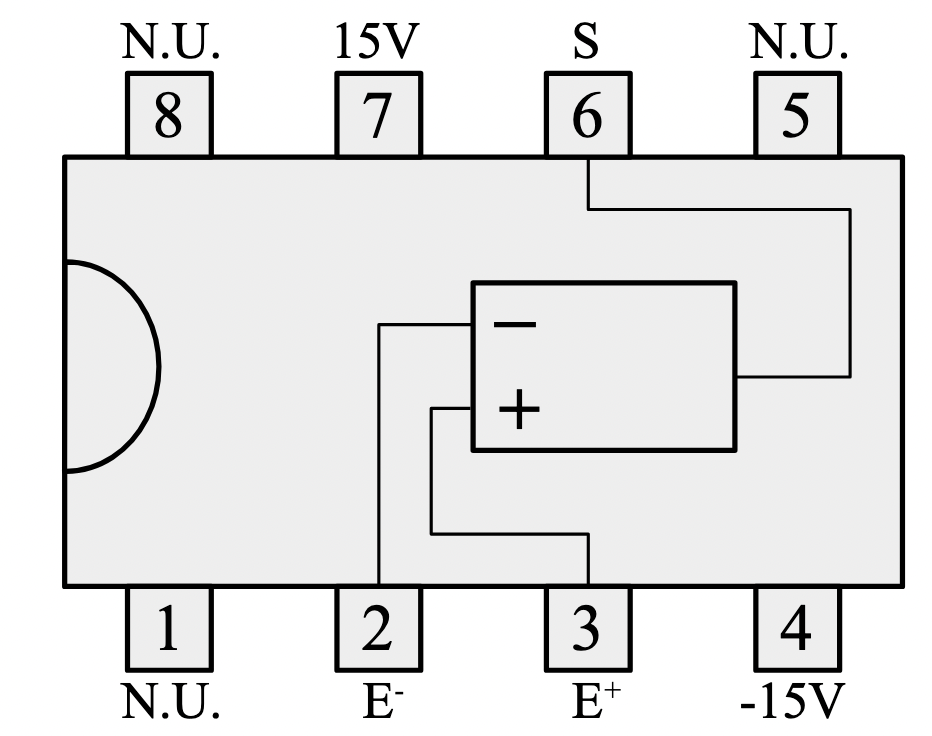
\includegraphics[scale=0.27]{E8-cours-0-ALI.png}
\end{wrapfigure}
\noi
• \textbf{Bornes :}
\begin{itemize}
\item[2 :] entrée inverseuse, notée - ou $E^{-}$ ;
\item[3 :] entrée non inverseuse : + ou $E^{+}$ ;
\item[6 :] sortie : $S$ ;
\item[4 :] $-V_{CC}$ : - 15 V ;
\item[7 :] $+V_{CC}$ : + 15 V ;
\end{itemize}
\vspace{0.1cm}

Les 3 bornes NU sont non utilisées ou permettent un réglage (tension de décalage).
\vspace{0.1cm}

\noi
• \textbf{Schéma électrique :}


\hspace{3cm}
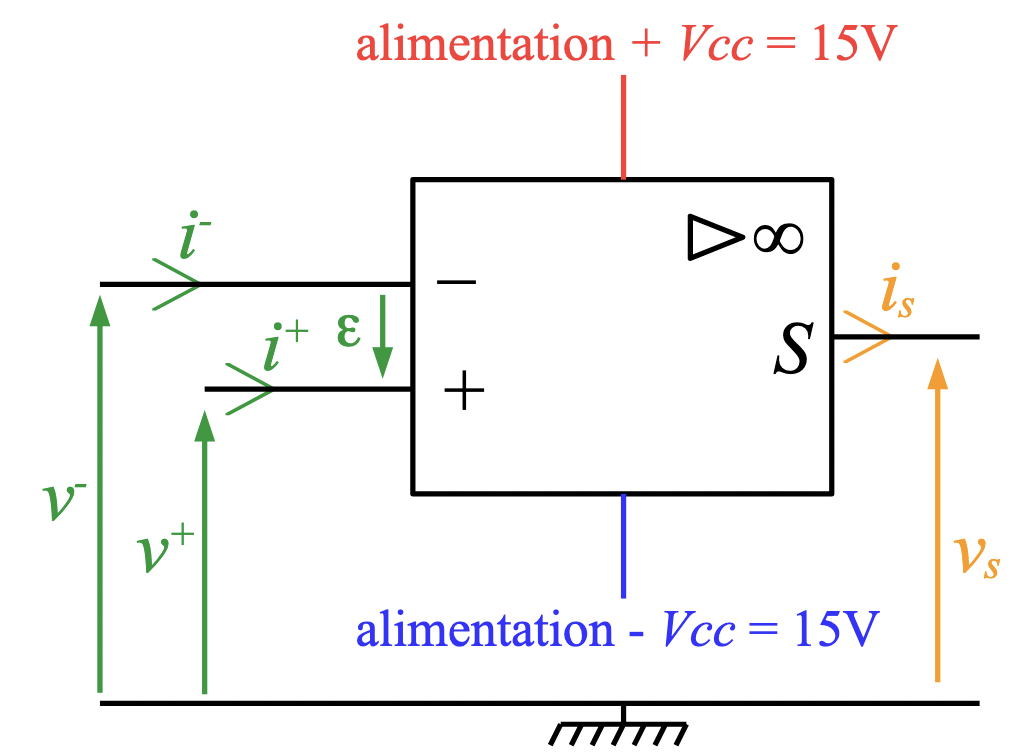
\includegraphics[scale=0.35]{E8-cours-0-schema-modele.png}
\esp

La masse de l'alimentation continue -15V / +15V doit être reliée à la masse du montage (il faut bien relier entre eux tous les points de masse).

L'alimentation n'est jamais représentée sur les schémas mais elle est bien présente dans les montages et il ne faut pas oublier de l'allumer.
\esp

\noi
\att Bien faire attention  où sont les entrées + et - sur les schémas : selon les circuits, les auteurs, ... l'entrée + peut être représentée au-dessus de l'entrée - ou l'inverse.
\esp


\noi
\idee Les tensions d'entrée $v^+$ et $v^-$ s'expriment avec les potentiels $V^+$ à l'entrée + et $V^-$ à l'entrée - : ($V_{masse} = 0\ \volt$) 
\vspace{0.1cm}

\hspace{3cm}
$\d
\left\{
    \begin{array}{ll}
        v^{+} = V^{+} - V_{masse} = V^{+}\\
        v^{-} = V^{-} - V_{masse} = V^{-}
    \end{array}
\right.
$

\esp

\noi
• La \textbf{tension de sortie} est $v_{S} = V_{S} - V_{masse} = V_{S}$  ($V_S$ potentiel au point $S$).
\vspace{0.1cm}

\noi
Elle dépend de la tension $\varepsilon = V^+ - V^-$ :  l'ALI \og amplifie \fg{} le signal d'entrée 

$\varepsilon = v^{+} - v^{-} = V^{+} - V^{-}$.
\esp

\noi
• \textbf{Courants.}
\vspace{0.1cm}

Les courants d'entrée sont notés $i^{-}$ (à l'entrée inverseuse $E^-$) et $i^{+}$ (à l'entrée non inverseuse $E^+$).

Le courant de sortie est $i_{S}$ (en général on ne le connait pas).



\subsection{\tb{Modèle de l'ALI idéal}}

\noi
• \textbf{Caractéristique de transfert :}
\vspace{0.1cm}
\begin{itemize}
\item[-] on trace $v_{S}$ en fonction de $\varepsilon = V^{+} - V^{-}$ en régime continu ;
\vspace{0.1cm}
\item[-] on voit apparaître les deux régimes de fonctionnement de l'ALI : le régime linéaire et le régime non linéaire (régime saturé) ;
\vspace{0.1cm}
\item[-] $+V_{sat}$ et $-V_{sat}$ sont appelées tensions de saturation.
\end{itemize}


\begin{center}
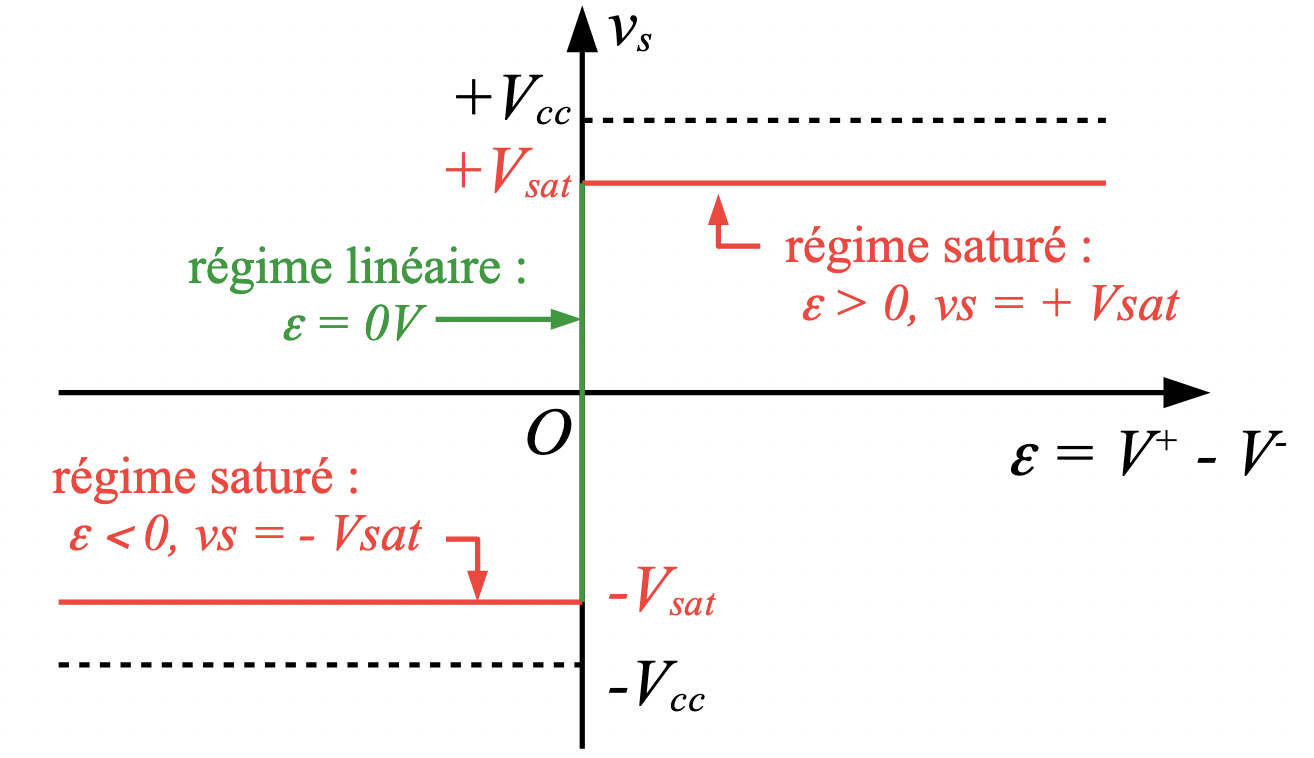
\includegraphics[scale=0.35]{E8-cours-0-fonction-transfert.png}
\end{center}

\begin{propriete}{ modèle de l'ALI idéal en régime linéaire - \co}{} 

L'\textbf{impédance d'entrée $Z_e$ est infinie} donc $i^+ = 0\ \ampere$ et $i^- = 0\ \ampere$.
\vspace{0.1cm}

\noindent
L'\textbf{impédance de sortie nulle} $Z_s = 0\ \ohm$ : l'ALI se comporte comme une source idéale de tension en sortie.
\vspace{0.1cm}

\noindent
En \textbf{régime linéaire} : $\varepsilon = V^+ - V^- = 0\ \volt$ soit $V^+ = V^-$.
\end{propriete}

\noi
• En régime non linéaire, $\varepsilon >0$ ($v_s = V_{sat}$) ou $\varepsilon < 0$ ($v_s =V_{sat}$). Les principaux montages utilisant des ALI en régime non linéaire sont des comparateurs (simple, à hystérésis, ...).


\section{\tr{Montages avec ALI en régime linéaire}}


\subsection{\tb{Généralités}}

\noi
• Rappel sur la \textbf{loi des nœuds en terme de potentiel}.
\esp
\esp

\begin{wrapfigure}[3]{r}{4cm}
\vspace{-1cm}
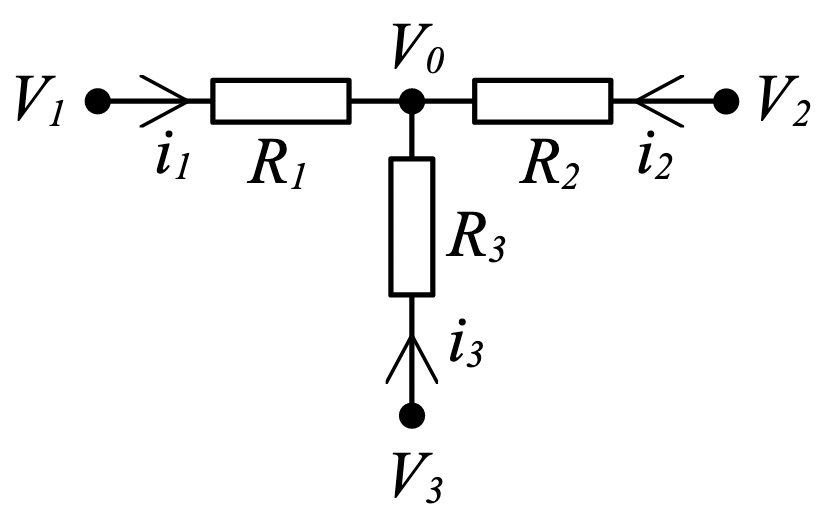
\includegraphics[scale=0.27]{E8-cours-0-millman.png} 
\end{wrapfigure}
Pour calculer $V^{+}$ et $V^{-}$ on utilise la loi des nœuds en terme de potentiel.

\noi
\exe $ \frac{V_1 - V_0}{R_1} + \frac{V_2 - V_0}{R_2} + \frac{V_3 - V_0}{R_3} = 0$ soit
 $\d V_{0} = \frac{\frac{V_{1}}{R_{1}} + \frac{V_{2}}{R_{2}}+ \frac{V_{3}}{R_{3}}}{\frac{1}{R_{1}} + \frac{1}{R_{2}}+ \frac{1}{R_{3}}}$.
\esp
\esp

\begin{methode}{étudier un montage avec un ALI idéal (régime linéaire)}{}
\r On calcule les potentiels $V^{+}$ et $V^{-}$ en appliquant la loi des nœuds en terme de potentiel aux entrées $E^{+}$ et $E^{-}$ de l'ALI idéal, avec des impédances complexes.
\vspace{0.1cm}

\noi
\r Les branches traversées par les courants d'entrées, d'intensités $i^{+} = 0A$ et $i^{-} = 0\ \ampere$, n'apparaissent pas dans la loi des nœuds, ces intensités étant nulles.
\vspace{0.1cm}

\noi
\r En régime linéaire on écrit ensuite $\so{V}^+ = \so{V}^-$; on déduit l'expression de $\so{v}_s$ puis de $v_s(t)$.
\end{methode}

\noi
\att On n'applique jamais la loi des nœuds en terme de potentiel à la sortie de l'ALI (on ne connait pas l'intensité de sortie $i_s$ de l'ALI).
\esp

\noi
• Rappel sur \textbf{l'impédance d'entrée d'un montage} .
\esp

\begin{definition}{impédance d'entrée d'un montage - \co}{}
On alimente un montage avec un générateur de fem $\so{v}_e(t)$ traversé par une intensité $\so{i}_e(t)$.
L'impédance d'entrée du montage est : 
\esp

\hspace{0.5cm}
$\d \so{Z}_e = \frac{\so{v}_e}{\so{i}_e}$  \hspace{0.3cm} (en CR par rapport au montage).

\vspace{-1.2cm}
\hspace{8cm}
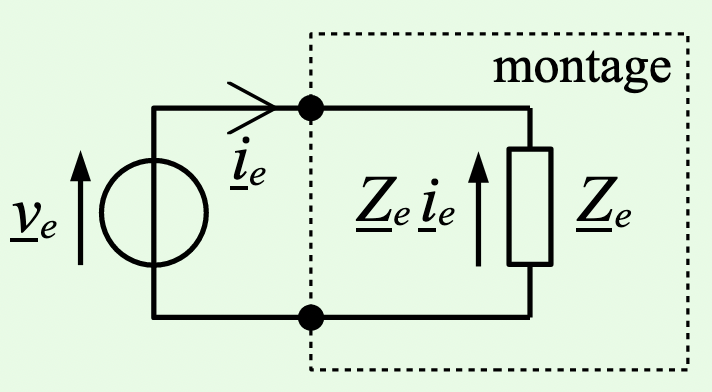
\includegraphics[scale=0.35]{E8-cours-0-Ze.png}
\end{definition}

\begin{methode}{déterminer l'impédance d'entrée d'un montage avec ALI}{}

\r Repérer la tension d'entrée $v_e$ délivrée par le générateur.
\esp

\noindent
\r Placer l'intensité $i_e$ circulant dans la branche du générateur.
\esp

\noindent
\r  Calculer $\d \so{Z}_e = \frac{\so{v}_e}{\so{i}_e}$ ($\so{Z}_e$ définie avec une convention récepteur par rapport au montage).

%\hspace{2cm}
%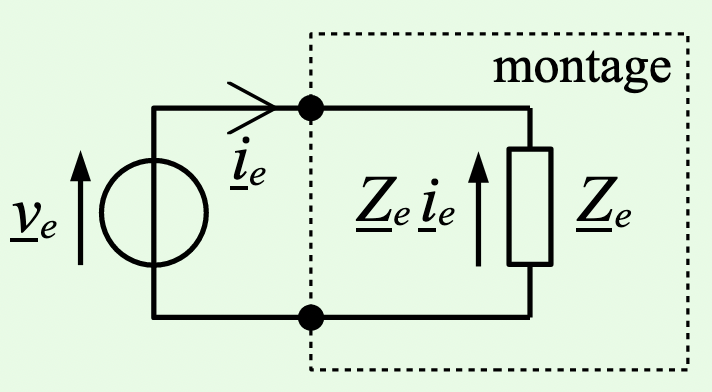
\includegraphics[scale=0.4]{E8-cours-0-Ze.png}
\end{methode}
%%
%\vspace{-0.4cm}
%

\esp

\noi
• \textbf{Boucle de rétroaction.}
\vspace{0.1cm}

Les boucles de rétroaction sont fondamentales dans les montages avec les ALI. Il faut bien les analyser : constitution, retour sur l'entrée inverseuse $E^-$ ou sur l'entrée non inverseuse $E^+$ ?
\vspace{0.1cm}

\begin{definition}{ boucle de rétroaction d'un montage avec ALI - \co}{}
Une boucle de rétroaction est une \textbf{partie de circuit}, constituée par un fil, un ou plusieurs dipôles, \textbf{partant de la sortie} $S$ et \textbf{revenant sur l'entrée inverseuse} $E^-$ ou sur l'\textbf{entrée non inverseuse} $E^+$ .
\end{definition}

\subsection{\tb{Réalisation de montages avec un ALI}}

Les montages peuvent être réalisés sur des plaquettes avec des ALI protégés dans des boitiers, les bornes étant nommées.
\esp

On utilise aussi des plaquettes d'essai d'électronique (bread board) : attention aux branchements !
\esp

\hspace{0.5cm}

\includegraphics[scale=0.33]{E8-cours-0-bread-board.png}


\subsection{\tb{Montage amplificateur non inverseur}}

\subsubsection{Montage théorique}

\noi
• \textbf{Schéma.}

\vspace{-0.5cm}
\hspace{3cm}
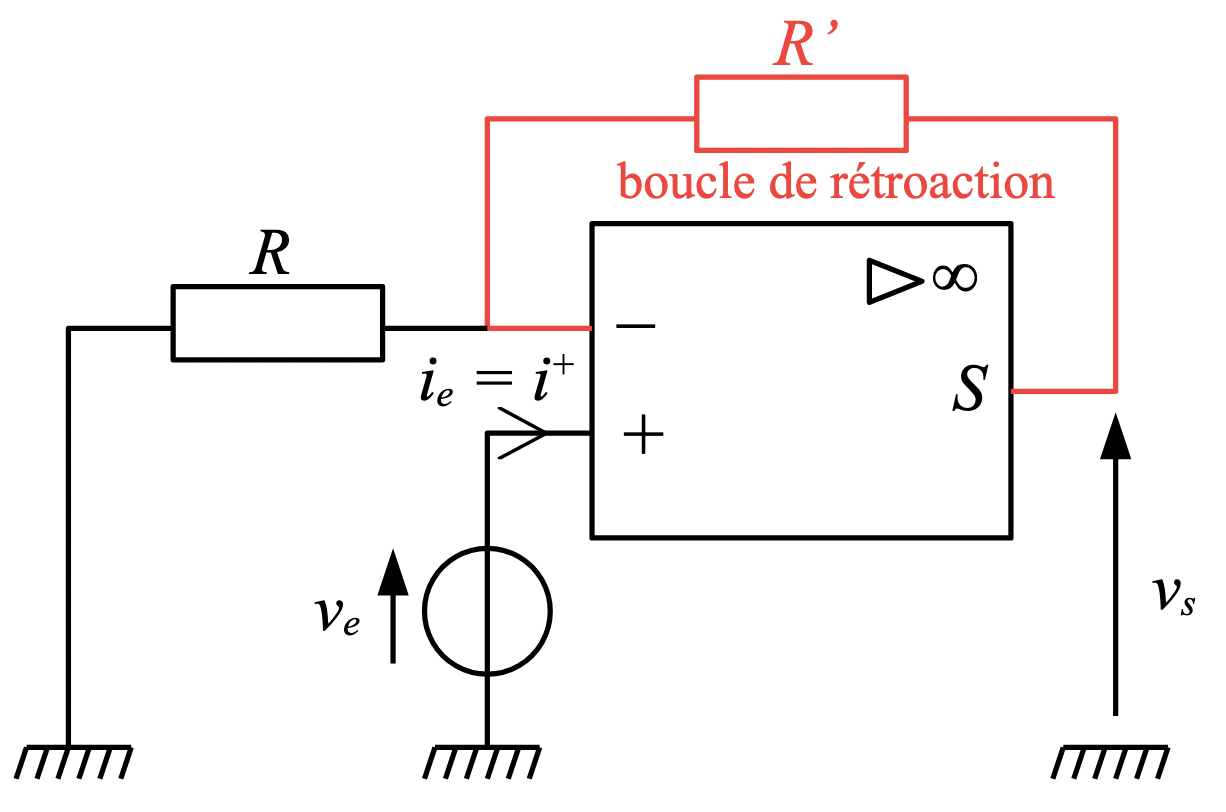
\includegraphics[scale=0.35]{E8-cours-0-non-inverseur.png}
\esp

\noi
• \textbf{Fonction de transfert.}
\esp

À l'entrée $E^+$ : $V^+ = v_e$.
\esp

Loi des nœuds en terme de potentiel à l'entrée $E^-$ : $\d \frac{0 - V^-}{R} + \frac{v_s - V^-}{R'} = 0$


soit $\d V^- = \frac{\dfrac{0}{R}+ \dfrac{v_s}{R'}}{\dfrac{1}{R} +\dfrac{1}{R'}} = \frac{R}{R+R'}v_s$.
\esp

Régime linéaire : $V^+ = V^-$ donc $\d v_e = \frac{R}{R+R'}v_s$ et
$\d v_s = \frac{R+R'}{R}v_e = \left(1 + \frac{R'}{R}\right)v_e$.
\esp

Fonction de transfert : $\d \so{H} = \frac{\so{v}_s}{\so{v}_e} = 1 + \frac{R'}{R}$.
\esp

\noi
• \textbf{Intérêt :} on obtient un signal de sortie identique au signal d'entrée mais avec une amplitude multipliée par $\d \left(1 + \frac{R'}{R}\right)$.
\esp

\noi
• \textbf{Impédance d'entrée :} le générateur est branché sur l'entrée $E^+$, donc  $i_e = i^+$. Ainsi : $\d \so{Z}_e = \frac{\so{v}_e}{\so{i}_e} = \frac{\so{v}_e}{\so{i}^+} \rightarrow \infty$ car $i^+ = 0\ \ampere$.
\esp

\begin{relation}{ montage amplificateur non inverseur - \co}{}
Fonction de transfert : $\d \so{H} = \frac{\so{v}_s}{\so{v}_e} = 1 + \frac{R'}{R}$.  Impédance d'entrée : 
$\d \so{Z}_e = \frac{\so{v}_e}{\so{i}^+} \rightarrow \infty$.
\end{relation}

\vspace{-0.2cm}

\subsubsection{Étude expérimentale}

\color{blue}
\noi
• \textbf{Réglages 1.} Réaliser le montage sur la plaquette d'essai en prenant :
\begin{itemize}
\item[-] $v_e(t) = V_{em}\cos(\omega t)$ avec $f = 1\ \kilo\hertz$ et $V_{em} = 0,5\ \volt$ ;
\item[-] $R = 1\ \kilo\ohm$ et $R' = 10\ \kilo\ohm$.
\end{itemize}
\esp

\color{black}

\noi
• \textbf{Observations.} 
\vspace{0.1cm}

On observe $v_s(t) \approx 11\times v_e(t)$ soit $\d v_s(t) = \left(1 + \frac{R'}{R}\right)v_e(t) = 11v_e(t)$.


\hspace{2.5cm}
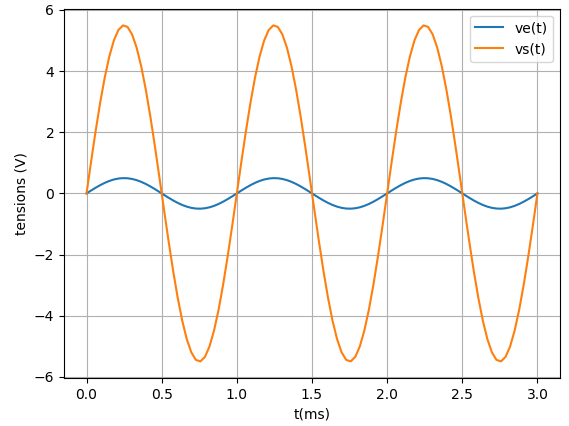
\includegraphics[scale=0.48]{AO-non-inverseur-c1.png} 


\noi
\color{blue}
• \textbf{Réglages 2.} On réalise maintenant le montage en prenant comme réglages :
\begin{itemize}
\item[-] $v_e(t) = V_{em}\cos(\omega t)$ avec $f = 1\ \kilo\hertz$ et $V_{em} = 3\ \volt$ ;
\item[-] $R = 1\ \kilo\ohm$ et $R' = 10\ \kilo\ohm$.
\end{itemize}
\esp

\color{black}

\noi
• \textbf{Observations.} 
\vspace{0.1cm}

Il y a écrétage à $+15\ \volt$ et $-15\ \volt$ environ car la tension de sortie $v_s(t)$ de l'ALI est limitée par les tensions d'alimentation $+V_{cc}$ et $-V_{cc}$. Or $11\times V_{em} = 33\ \volt > 15\ \volt$ ...

On dit que l'ALI fonctionne en régime saturé (régime non linéaire : on a une tension sinusoïdale à l'entrée mais la tension de sortie ne l'est pas).
\esp

\hspace{2.7cm}
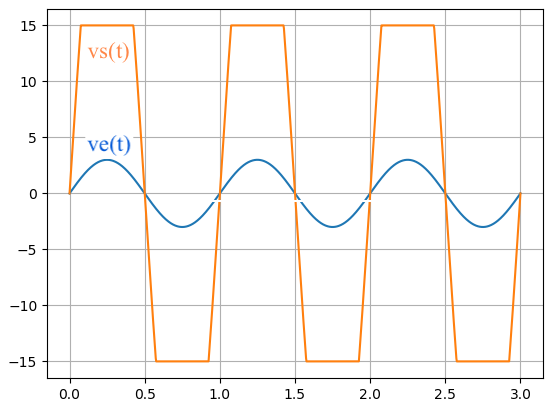
\includegraphics[scale=0.48]{AO-non-inverseur-c2.png} 
\esp

\noi
• \textbf{Diagramme de Bode du gain.}
\vspace{0.1cm}
%
%\meth{ M3 : tracer des courbes  $G_{\deci\bel}(f)$ et $\varphi (v_s/v_e)$ .}
%{\esp
%
%\r Brancher la tension d'entrée $v_e$ sur la voie 1 de l'oscilloscope et la tension de sortie $v_s$ sur la voie 2.
%
%\noindent
%\r Effectuer un balayage rapide en fréquence pour observer le comportement du circuit (type de filtre, ordre de grandeur des fréquences caractéristiques (pic, début de la décroissance pour un filtre passe-bas, du plateau pour un filtre passe-haut).
%
%\noindent
%\r Débuter les mesures à basses fréquences : relever $V_{em}$ (ou $V_{e,eff}$) et $V_{sm}$ (ou $V_{s,eff}$) ainsi que $\varphi (v_s/v_e)$ (attention au signe) à l'oscilloscope.
%
%\noindent
%\r Choisir les valeurs des fréquences pour pouvoir tracer les asymptotes et les points particuliers.
%
%\noindent
%\r Vérifier constamment que les deux courbes ($v_e(t)$ et $v_s(t)$) sont des sinusoïdes (si ce n'est pas le cas, adapter l'amplitude de la tension d'entrée) en raisonnant en échelle logarithmique.
%
%\noindent
%\r Pour chaque fréquence calculer $\d G_{\deci\bel} = 20\ log\left(\frac{V_{sm}}{V_{em}}\right)$ (ou avec les valeurs efficaces).
%
%\noindent
%\r Placer les points sur le papier semi-logarithmique.
%}


\tb{Mesures : tracer à l'aide du logiciel Oscille 5 le diagramme de Bode jusqu'à $80\ \kilo\hertz$ du gain $\d G_{\deci\bel} = 20\times log\left(\left\vert \frac{\so{v}_s}{\so{v}_e} \right\vert \right)$ de ce montage pour $R = 1\ \kilo\ohm$ et $R' = 10\ \kilo\ohm$.}



\begin{center}
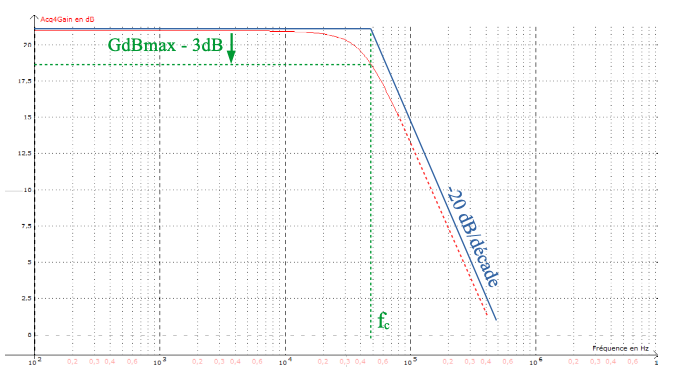
\includegraphics[scale=0.5]{E8-tp-GdB-passe-bas.png} 
\end{center}


\test {\small \textit{Déduire du diagramme de Bode du gain le type de la fonction de transfert $\so{H}$ de ce montage avec un ALI réel. Quel est le défaut mis en évidence ici ?}}

\subsubsection{Boucle de rétroaction}

\noi
• \textbf{Boucle de rétroaction :} il s'agit ici de la branche constituée par $R'$, qui relie la sortie de l'ALI à l'entrée non inverseuse $E^+$.
\esp

\color{blue}
\noi
• \textbf{Montage :} on inverse les branchements du montage non inverseur aux entrées $E^{+}$ et $E^{-}$, ainsi la boucle de rétroaction va revenir sur l'entrée $E^{+}$. 
\esp

\hspace{2cm}
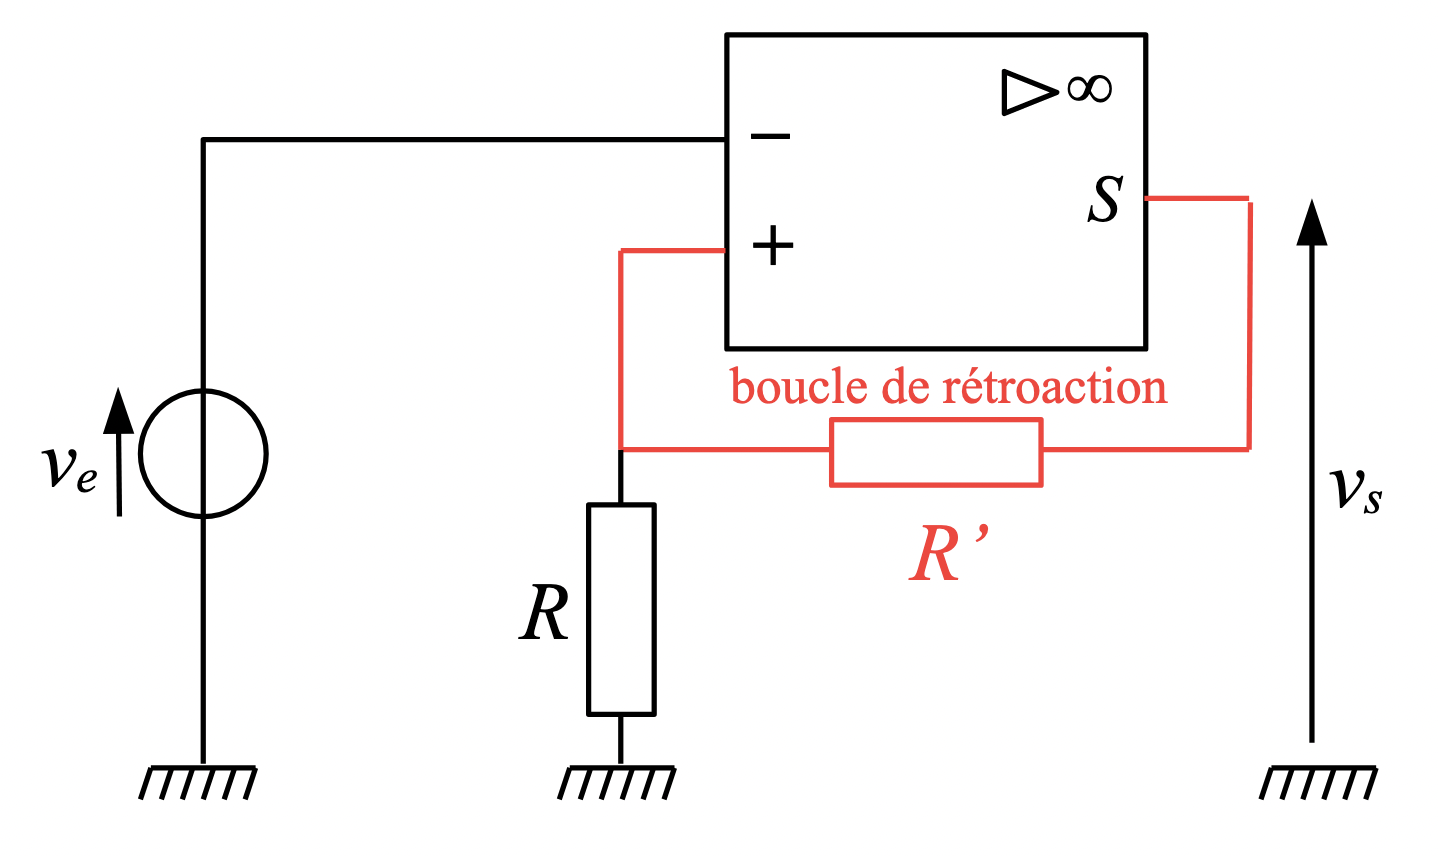
\includegraphics[scale=0.3]{E8-cours-0-ALI-sat.png}

\color{black}
En gardant les réglages 2 on constate que la tension de sortie $v_s(t)$ de l'ALI n'est plus sinusoïdale :  l'ALI fonctionne en régime non linéaire.

Les relations écrites précédemment ne peuvent plus l'être et on étudie le montage en raisonnant un peu différemment, même si on écrit la loi des nœuds en terme de potentiel aux entrées de l'ALI.
\esp

\begin{propriete}{régime linéaire - \co}{}
Lorsque la \textbf{boucle de rétroaction} est branchée sur l'\textbf{entrée non inverseuse} $E^-$ et que l'ALI est en \textbf{régime non saturé}, il fonctionne en \textbf{régime linéaire} et $V^+ = V^-$.
\end{propriete}

%\vspace{-0.2cm}

\subsection{\tb{Montage suiveur}}

\noi
• \textbf{Montage théorique :}

\vspace{-0.4cm}
\hspace{4cm}
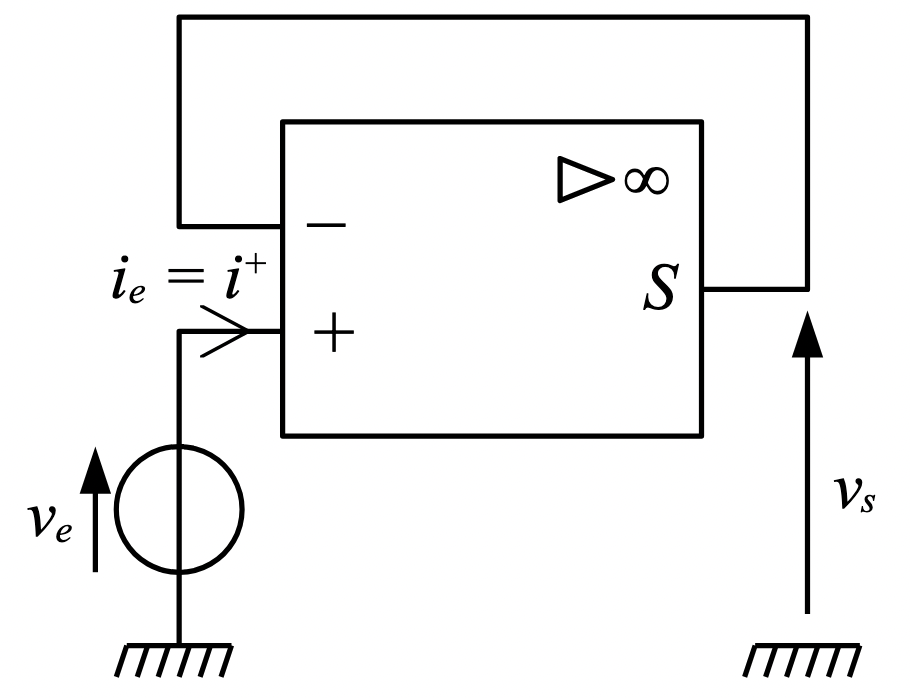
\includegraphics[scale=0.3]{E8-cours-0-suiveur.png}


\noi
• \textbf{Expression de $v_s$ :}
\vspace{0.1cm}
\begin{itemize}
\item[-] $v_e = V^{+}$ et $v_s = V^{-}$ ;
\vspace{0.1cm}
\item[-] la boucle de rétroaction est branchée sur l'entrée inverseuse donc l'ALI fonctionne en régime linéaire : $\varepsilon = V^{+} - V^{-} = 0\ \volt$ ;
\vspace{0.1cm}
\item[-] on conclut : $v_s = v_e$.
\end{itemize}
\esp

\noi
• \textbf{Intérêt :} l'ALI en sortie, se comporte comme une source idéale de tension. On obtient donc un signal $v_s$ image de $v_e$, mais sans les inconvénients de la résistance interne de la source engendrant $v_e$.
\esp

\noi
• \textbf{Impédance d'entrée :} $\d \so{Z}_e = \frac{\so{v}_e}{\so{i}_e} \rightarrow \infty$ car $i_e = i^+ = 0\ \ampere$.
\esp

\begin{relation}{ montage suiveur avec ALI idéal - \co}{} 
Fonction de transfert : $\d \so{H} = \frac{\so{v}_s}{\so{v}_e} = 1$. 
Impédance d'entrée : 
$\d \so{Z}_e = \frac{\so{v}_e}{\so{i}^+} \rightarrow \infty$.
\end{relation}


\subsection{\tb{Montage intégrateur}}

\subsubsection{Montage théorique}

\noi
• \textbf{Schéma :}

\vspace{-0.4cm}
\hspace{2.5cm}
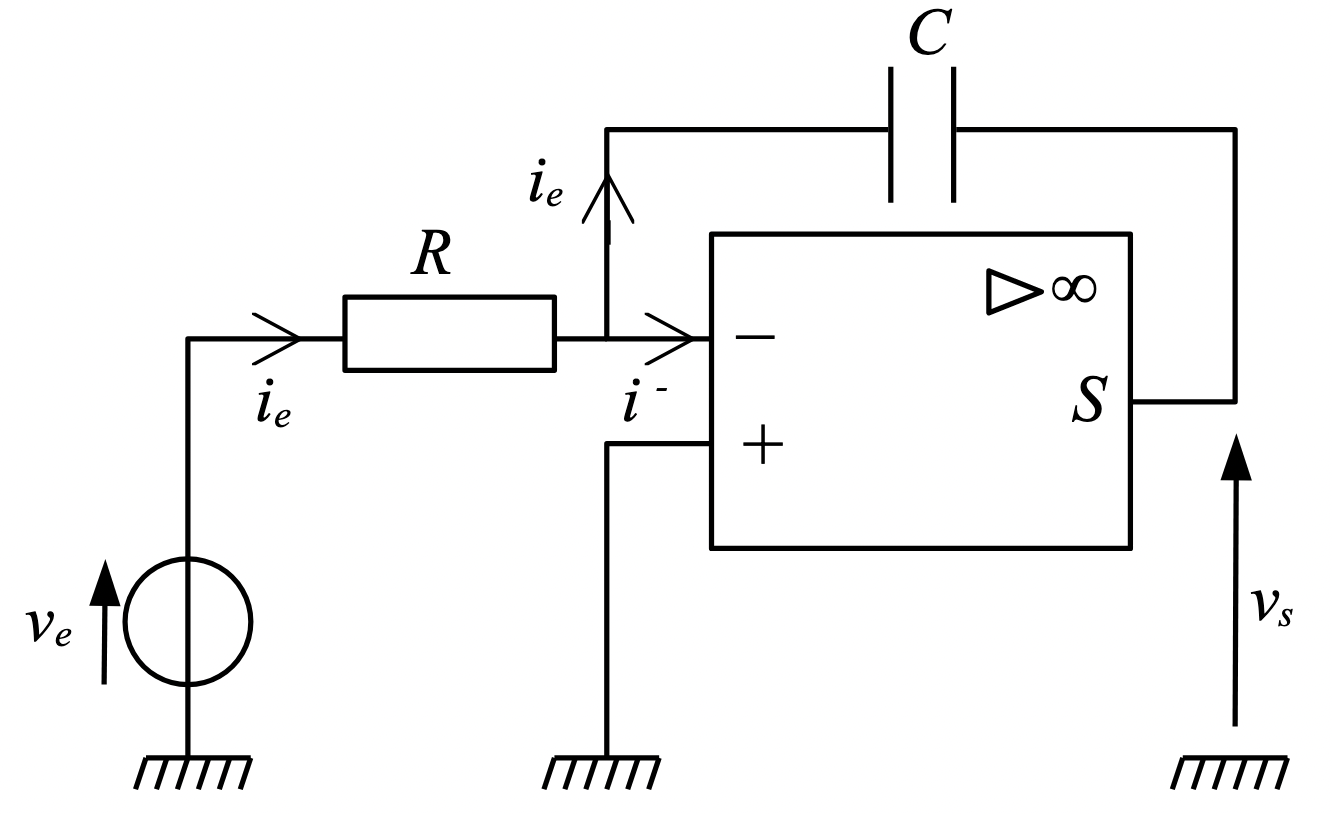
\includegraphics[scale=0.3]{E8-cours-0-integrateur.png}
\esp

\test {\small \textit{Montrer, en appliquant la loi des nœuds en terme de potentiel, que l'on obtient le résultat suivant, l'ALI fonctionnant en régime linéaire : $\d v_s(t) = -\frac{1}{RC}\int v_e(t)\ dt$.}}
\esp

\noi
• \textbf{Impédance d'entrée :}
\vspace{0.1cm}
\begin{itemize}
\item[-] pour l'ALI idéal : $i^- = 0\ \ampere$ ;
\vspace{0.1cm}
\item[-] loi des mailles pour la maille $masse\ -\ E^-\ -\ E^+\ -\ masse$ : 

$v_e -Ri_e + (V^+ - V^-) = 0$ or en régime linéaire $\varepsilon = V^+ - V^- = 0\ \volt$ donc $v_e = Ri_e$ ;
\vspace{0.1cm}
\item[-] on conclut : $\d \so{Z}_e = \frac{\so{v}_e}{\so{i}_e} = R$.
\end{itemize}
\esp

\begin{relation}{montage intégrateur avec ALI idéal - \co}{} 
Fonction de transfert : $\d \so{H} = \frac{\so{v}_s}{\so{v}_e} = -\frac{1}{jRC\omega}$. Impédance d'entrée : 
$\d \so{Z}_e =R$.
\end{relation}

\test {\small \textit{En étudiant la fonction de transfert $\d \so{H} = \frac{\so{v}_s}{\so{v}_e}$ montrer que des signaux de certains fréquences peuvent poser problème.}}


\subsubsection{Étude expérimentale}

\color{blue}
\noi
• \textbf{Réglages :} $ R = 1\ \kilo\ohm$, $C = 100\ \nano\farad$, $f = 1\ \kilo\hertz$ et $V_{em} = 0,5\ \volt$. Choisir $v_e(t)$ sinusoïdale, triangulaire et en créneau. L'oscilloscope est réglé en AC.
\esp

\color{black}
\noi
• \textbf{Observations.}
\vspace{0.1cm}

On constate que le montage intègre bien et change le signe (sinusoïde : $v_s(t)$ en avance de $\frac{\pi}{2}\ \radian$ sur $v_e(t)$ car intégrer engendre un retard de $\frac{\pi}{2}\ \radian$ et multiplier par - ajoute $\pi\ \radian$) ; triangulaire : on observe des paraboles pour $v_s(t)$ ; pour les créneaux, des droites).
\vspace{0.1cm}

Le montage intègre aussi des grandeurs continues (tension de décalage à l'entrée de l'ALI par exemple) qui engendre un phénomène de dérive. On utilise souvent un montage pseudo-intégrateur en ajoutant une résistance en parallèle avec le condensateur.


\subsection{\tb{Montage inverseur}}


\subsubsection{Montage théorique}

\noi
• \textbf{Schéma :}

\hspace{2cm}
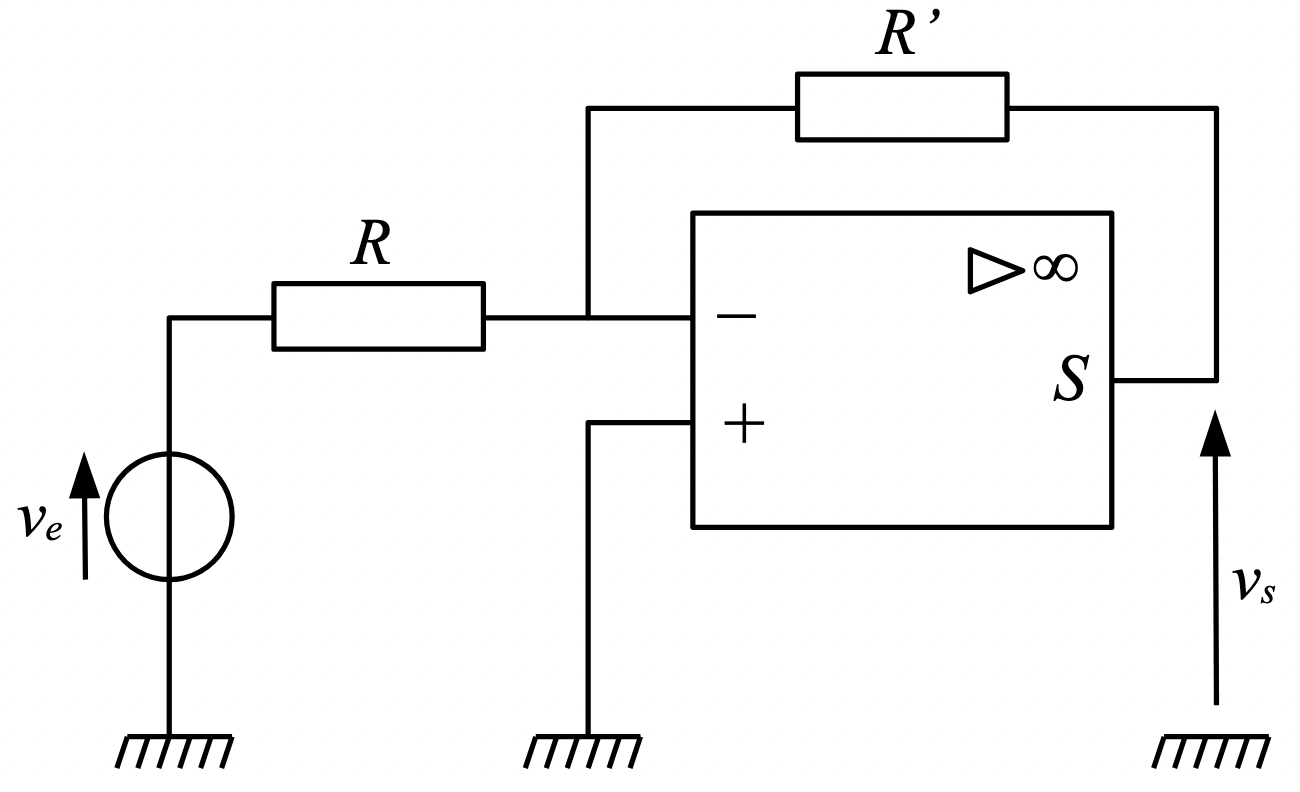
\includegraphics[scale=0.3]{E8-cours-0-inverseur.png}
\esp

\test {\small \textit{Déterminer l'expression de la fonction de transfert $\d \so{H} = \frac{\so{v}_s}{\so{v}_e}$.}}
\esp

\test {\small \textit{Déterminer l'expression de l'impédance d'entrée du montage $\d \so{Z}_e = \frac{\so{v}_e}{\so{i}_e}$.}}
\esp

\begin{relation}{montage inverseur avec ALI idéal - \co}{} 
Fonction de transfert : $\d \so{H} = \frac{\so{v}_s}{\so{v}_e} = -\frac{R'}{R}$. Impédance d'entrée : $\d \so{Z}_e = R$.
\end{relation}


\subsubsection{Étude expérimentale}

\color{blue}
\noi
• \textbf{Réglages :} $v_e(t) = V_{em}\ sin(\omega t)$ avec $f = 1\ \kilo\hertz$ et $V_{em} = 0,5\ \volt$  ; $R = 1\ \kilo\ohm$ et $R' = 10\ \kilo\ohm$.
\esp

\color{black}
\noi
• \textbf{Observations.}
\vspace{0.1cm}

On obtient 2 courbes en opposition de phase avec l'amplitude de $v_s(t)$ 10 fois plus grande que celle de $v_e(t)$.



\section{\tr{Filtres actifs passe-bande d'ordre 2}}

\noi
• \textbf{Montage :}


\hspace{1.5cm}
\begin{center}
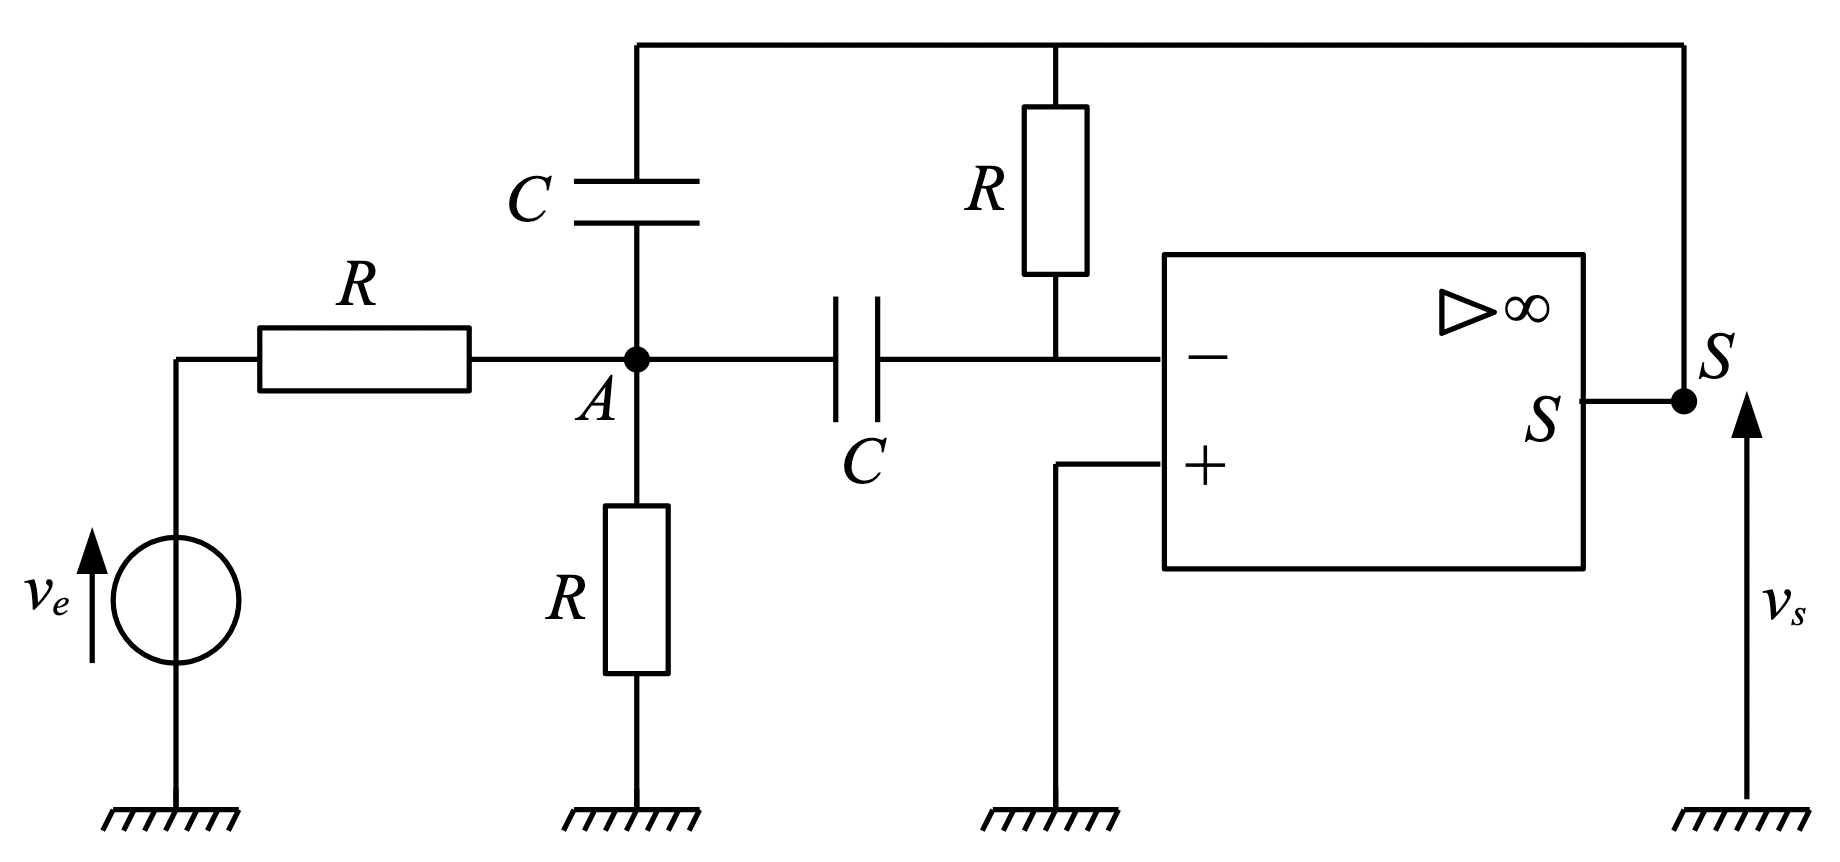
\includegraphics[scale=0.3]{E8-cours-0-passe-bande.png}
\end{center}
\esp

\noi
• \textbf{Théorie :}
\vspace{0.1cm}
\begin{itemize}
\item[-] la fonction de transfert est du type : $\d \so{H} = \frac{\so{v}_s}{\so{v}_e} = \frac{H_0}{1 + jQ\left(x-\frac{1}{x}\right)}$ avec $\d x = \frac{\omega}{\omega_0}$ ;
\vspace{0.1cm}
\item[-] on obtient : $\d \omega_0 = \frac{\sqrt{2}}{RC}$ soit  $\d f_0 = \frac{1}{\sqrt{2}\pi RC}$, $H_0 = -1/2$ et $Q = \frac{1}{\sqrt{2}}$.
\end{itemize}
\esp

\color{blue}
\noi
• \textbf{Mesures :} tracer à l'aide du logiciel Oscillo 5 le diagramme de Bode (entre 50 Hz et 50 kHz) pour  $R = 1\ \kilo\ohm$ et  $C = 100\ \nano\farad$.
\esp


\color{black}

\noi
• \textbf{Courbes :}


- gain $G_{\deci\bel}$ :

\begin{center}
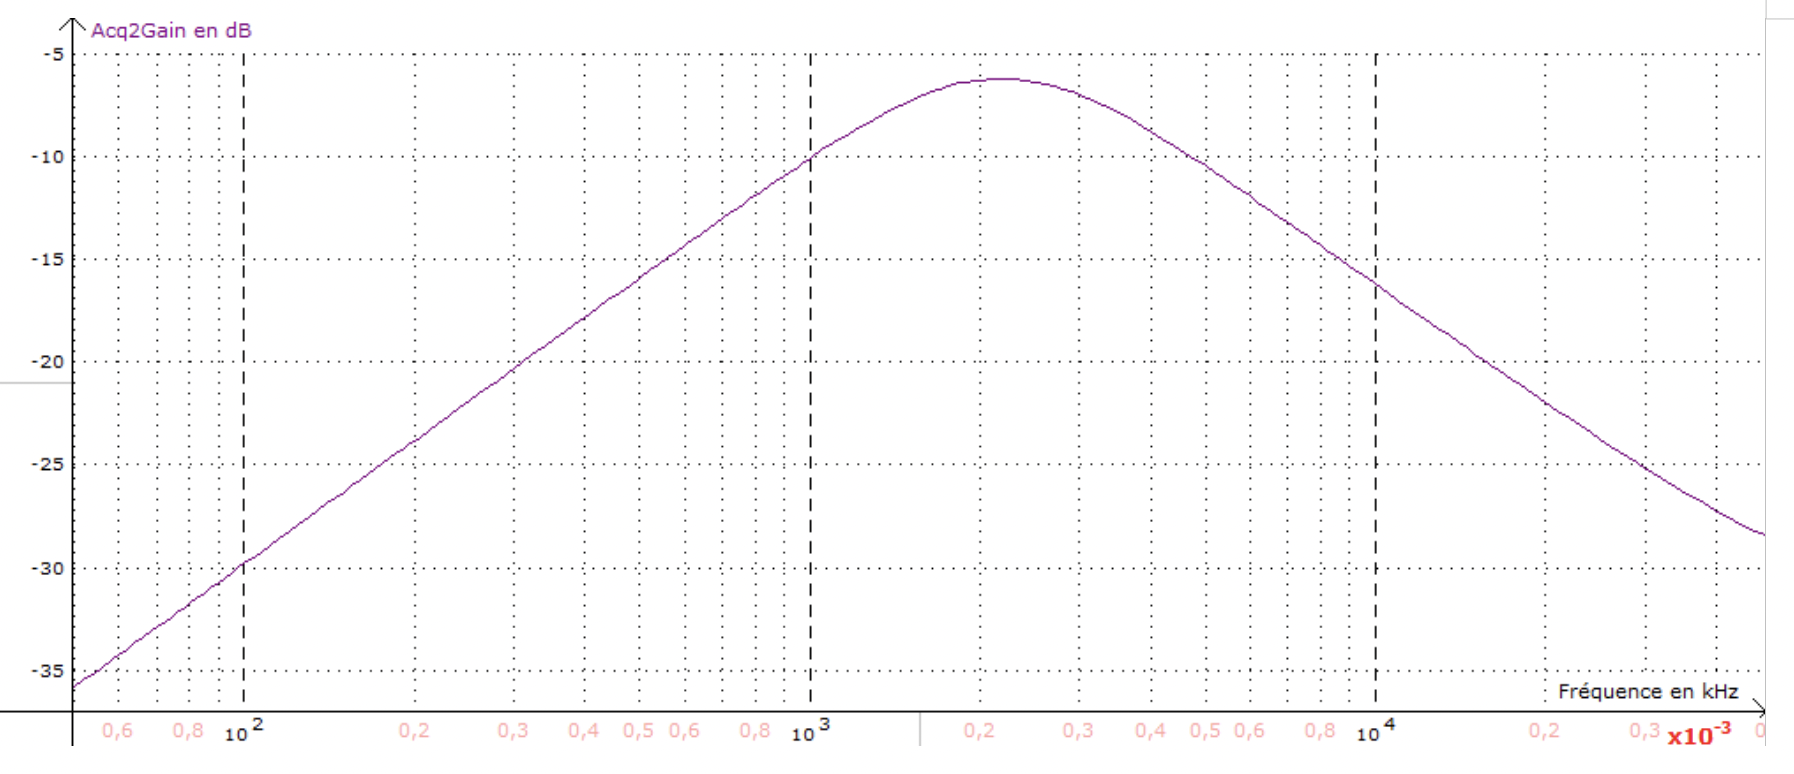
\includegraphics[scale=0.41]{E8-cours-0-gain-filtre-actif.png}
\end{center}

- phase (en radian) :

\begin{center}
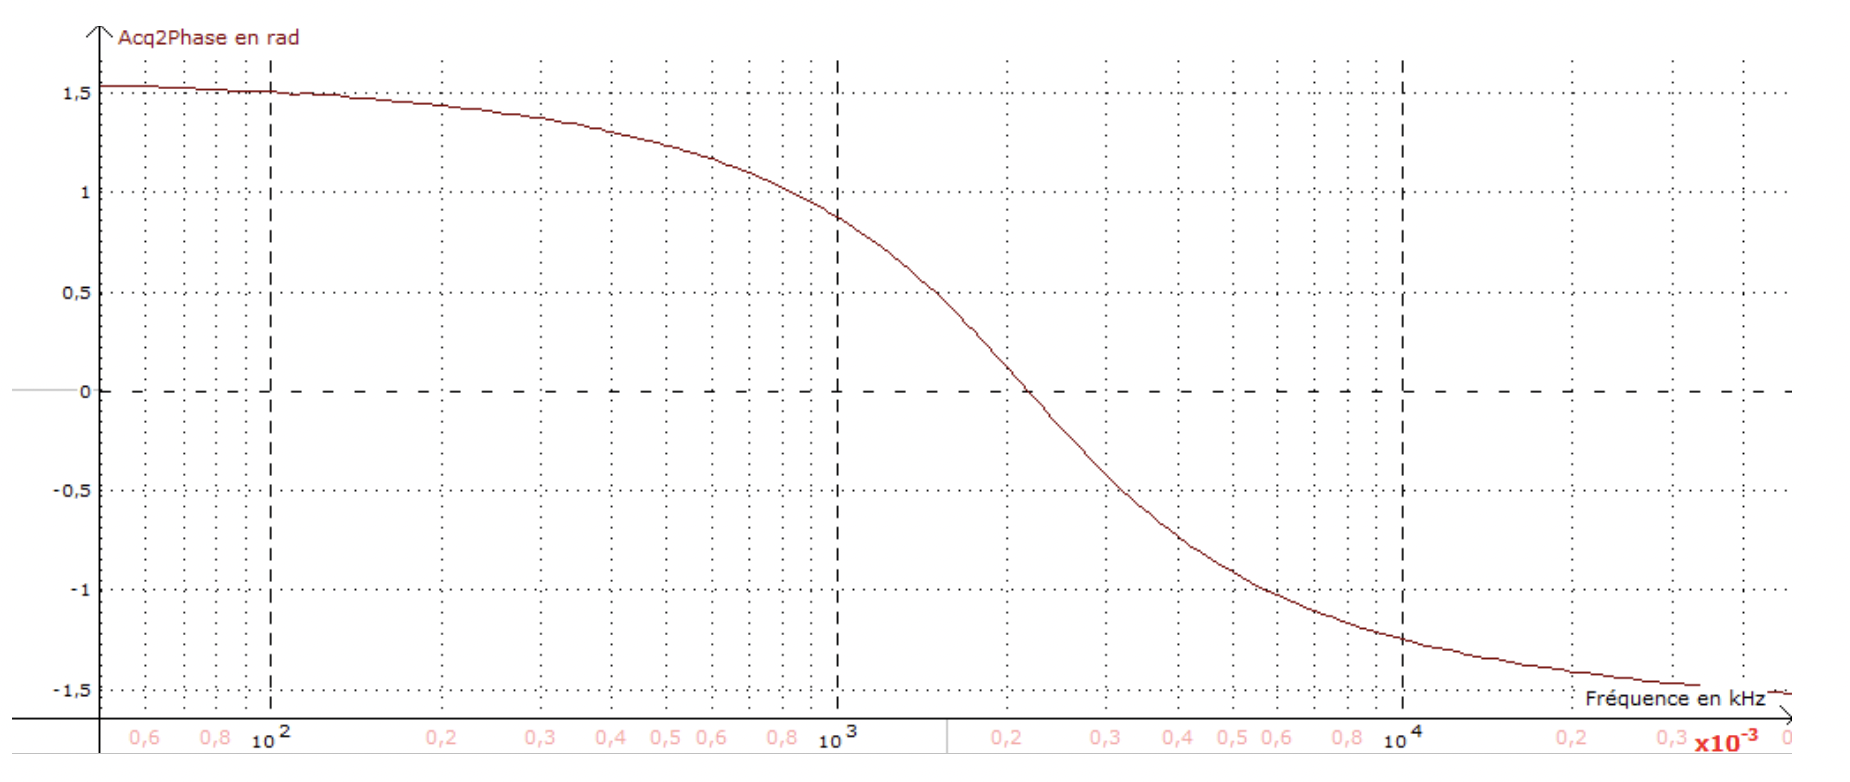
\includegraphics[scale=0.35]{E8-cours-0-phase-filtre-actif.png}
\end{center}



\noi
• \textbf{Exploitation :} déduire de la courbe du gain décibel courbes la fréquence centrale $f_0$ du filtre, les fréquences de coupure, la bande passante $\Delta f$, le facteur de qualité $Q$ et les pentes des asymptotes. Comparer aux valeurs théoriques.


\begin{center}
\begin{tabular}{|c|c|c||c|c|c|}
\hline 
 $f_{0,th}$  & $Q_{th}$ & $G_{\deci\bel max,th}$& $f_{0,exp}$ & $Q_{exp}$ &  $G_{\deci\bel max,exp}$ \\ 
\hline 
 2250  Hz & 0,71 & -6 dB & 2200 Hz & 0,69 & -6,2 dB \\ 
\hline 
\end{tabular} 
\end{center}


\noi
Il y a un bon accord entre le modèle et les valeurs expérimentales.
\esp

\noi
• \textbf{ Filtrage.}
\vspace{0.1cm}

\tb{Pour observer le filtrage, régler $v_e(t)$ (GBF) en signal en créneau avec les fréquences 100 Hz, 2250 Hz et 10 kHz pour les 2 valeurs de $k$}
\vspace{0.1cm}

\noindent
Pour un signal en créneau : $\d v_e(t) = \frac{4}{\pi}\left[sin(2\pi ft) + \frac{1}{3}sin(6\pi ft) + \frac{1}{5}sin(10\pi ft)+ ...\right]$. 
\esp

- Pour $f = 100\ \hertz$ on obtient les courbes temporelles :
\esp

\hspace{1cm}
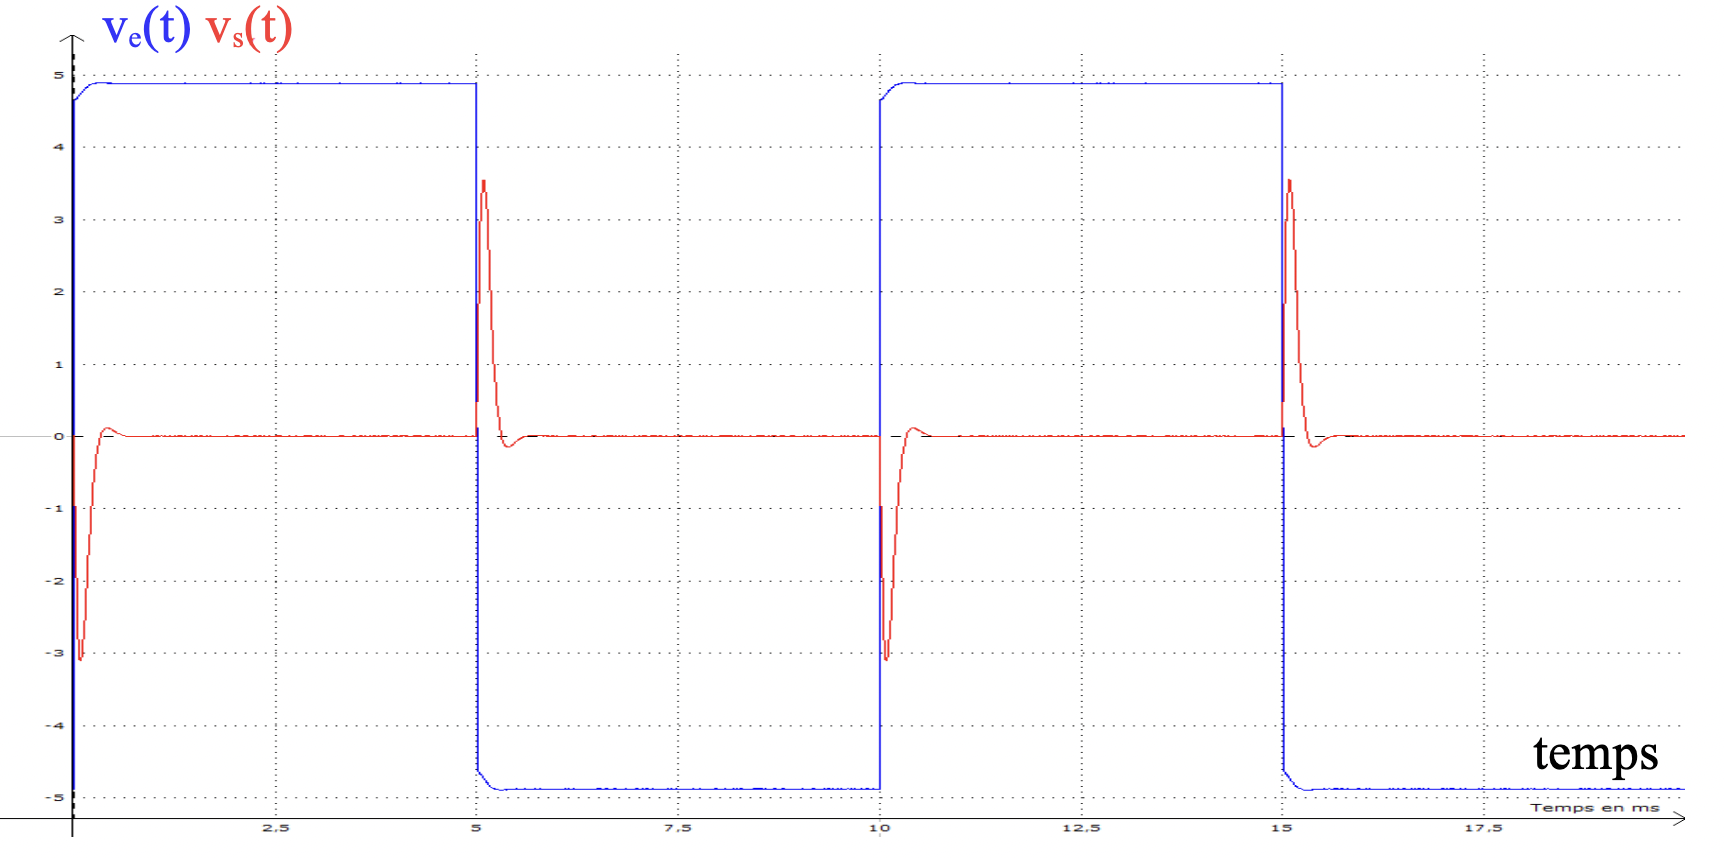
\includegraphics[scale=0.35]{filtre-actif-100-t.png}
\esp

Spectres des signaux d'entrée et de sortie :


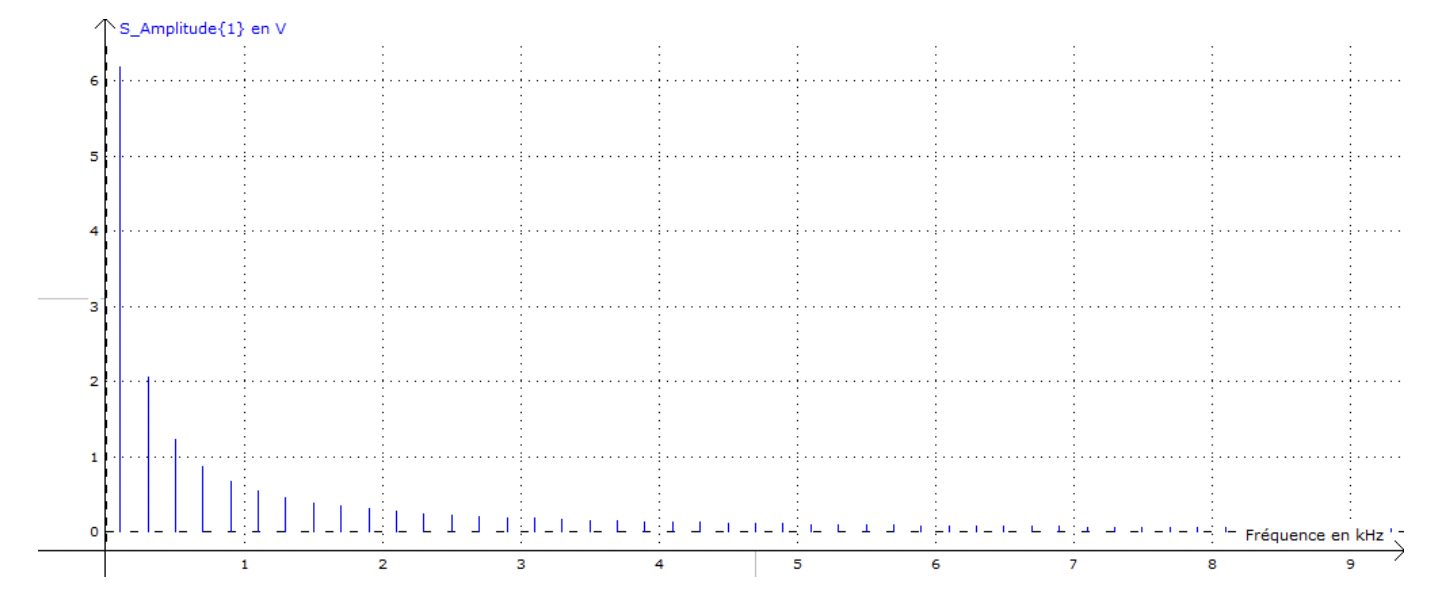
\includegraphics[scale=0.4]{filtre-actif-spectre-entree-100} 

\hspace{0.26cm}
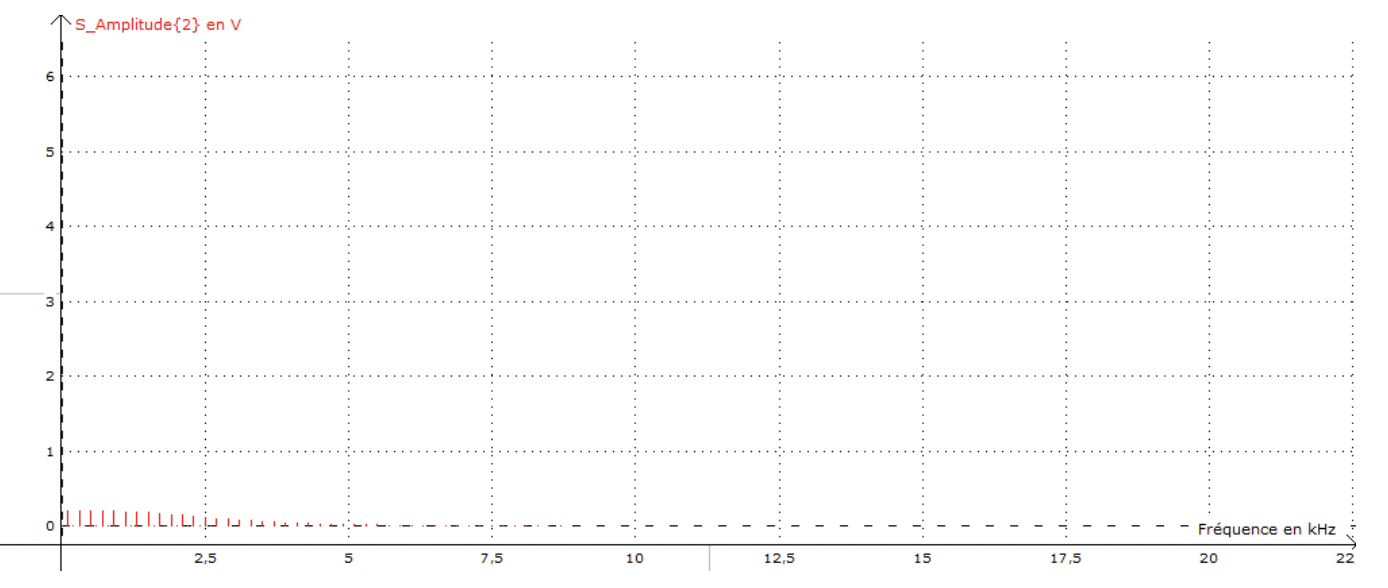
\includegraphics[scale=0.39]{filtre-actif-spectre-sortie-100} 

\esp

Toutes les composantes du signal d'entrée ayant une amplitude non négligeable sont dans la pente à + 20 dB / décade du diagramme du gain du filtre : le signal d'entrée est dérivé et l'on obtient des pics.

On peut aussi analyser le signal de sortie comme la réponse à des échelons de tension en régime pseudo-périodique avec faible facteur de qualité ($Q  \approx 0,7 > 0,5$).
\esp

- Pour $f = 2250\ \hertz$ on obtient les courbes temporelles :
\esp

\hspace{1cm}
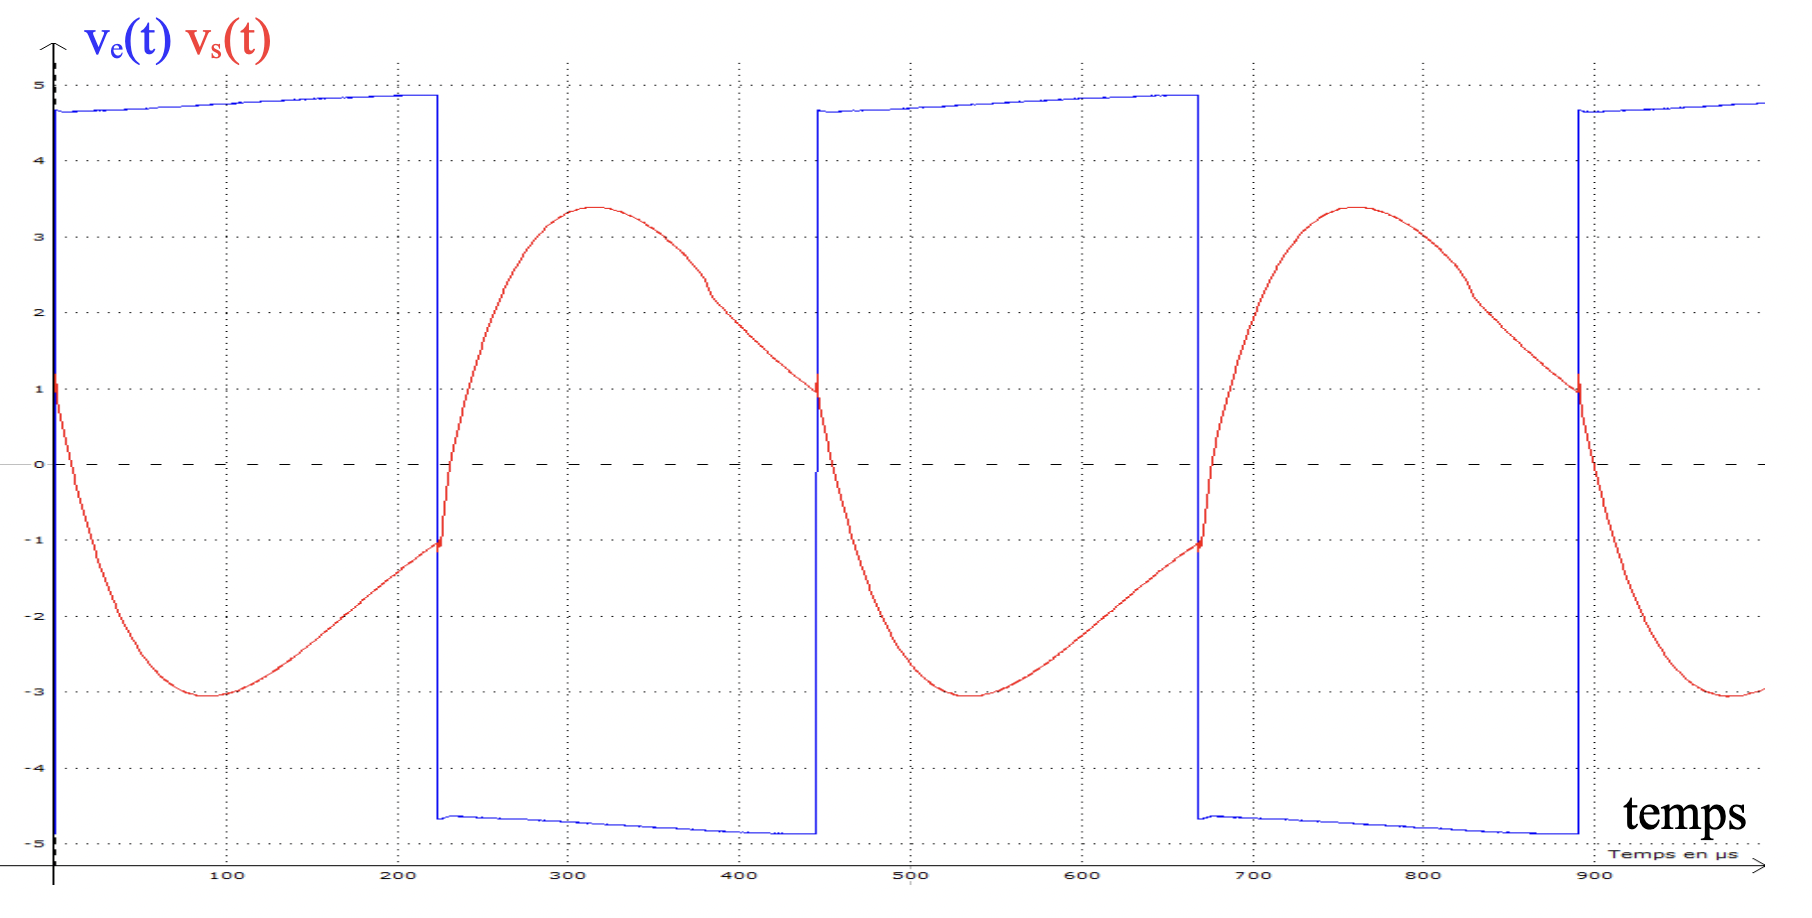
\includegraphics[scale=0.35]{filtre-actif-2250-t.png}
\esp

Spectres des signaux d'entrée et de sortie :


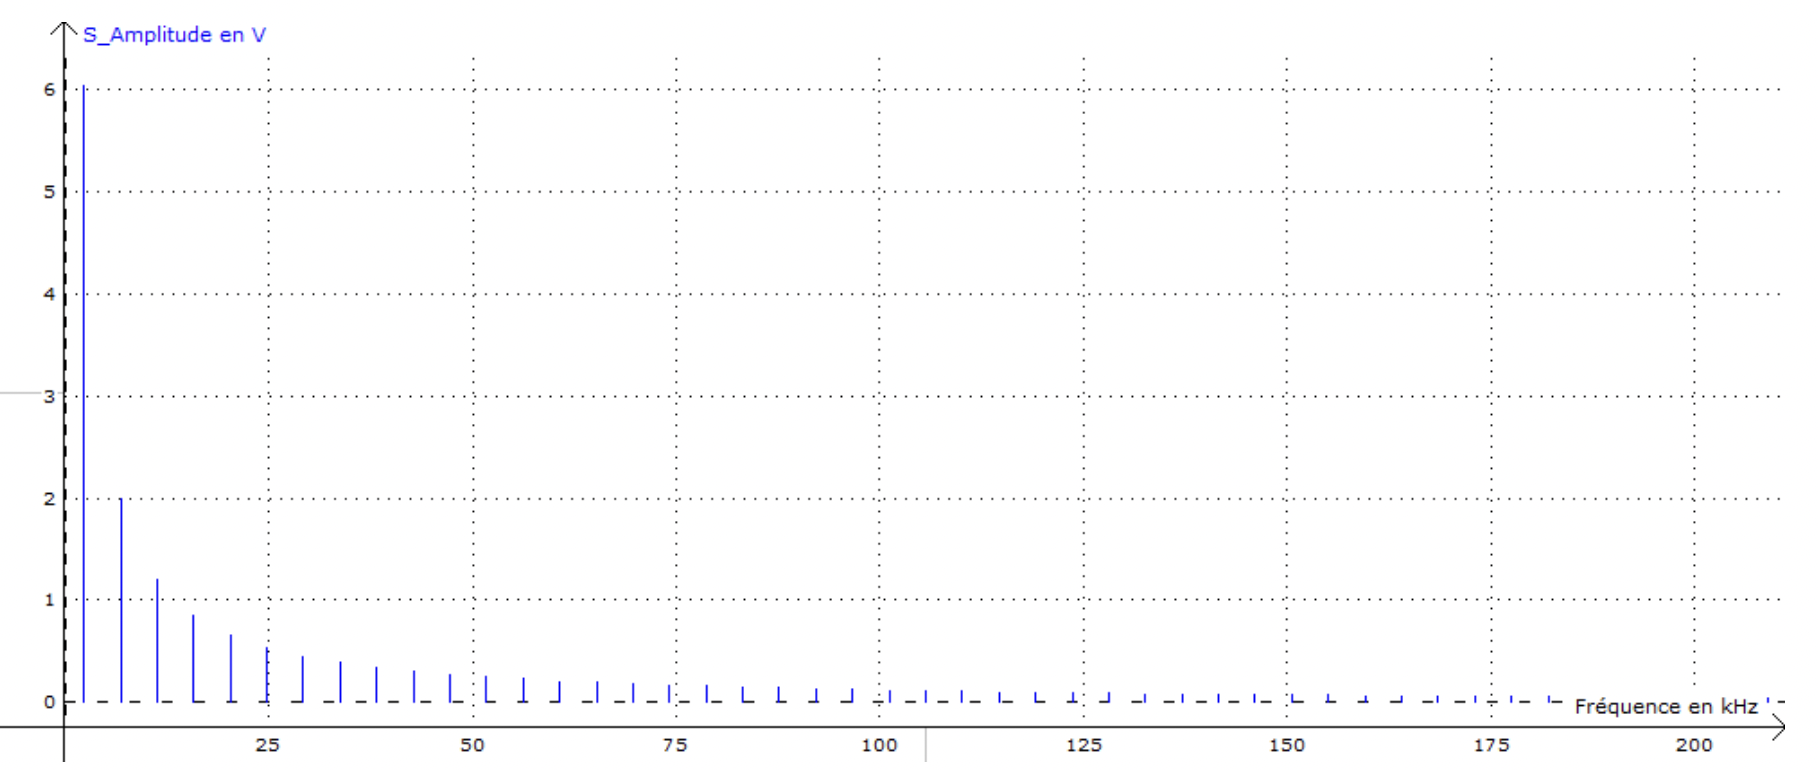
\includegraphics[scale=0.3]{filtre-actif-spectre-entree-2250} 

\hspace{-0.1cm}
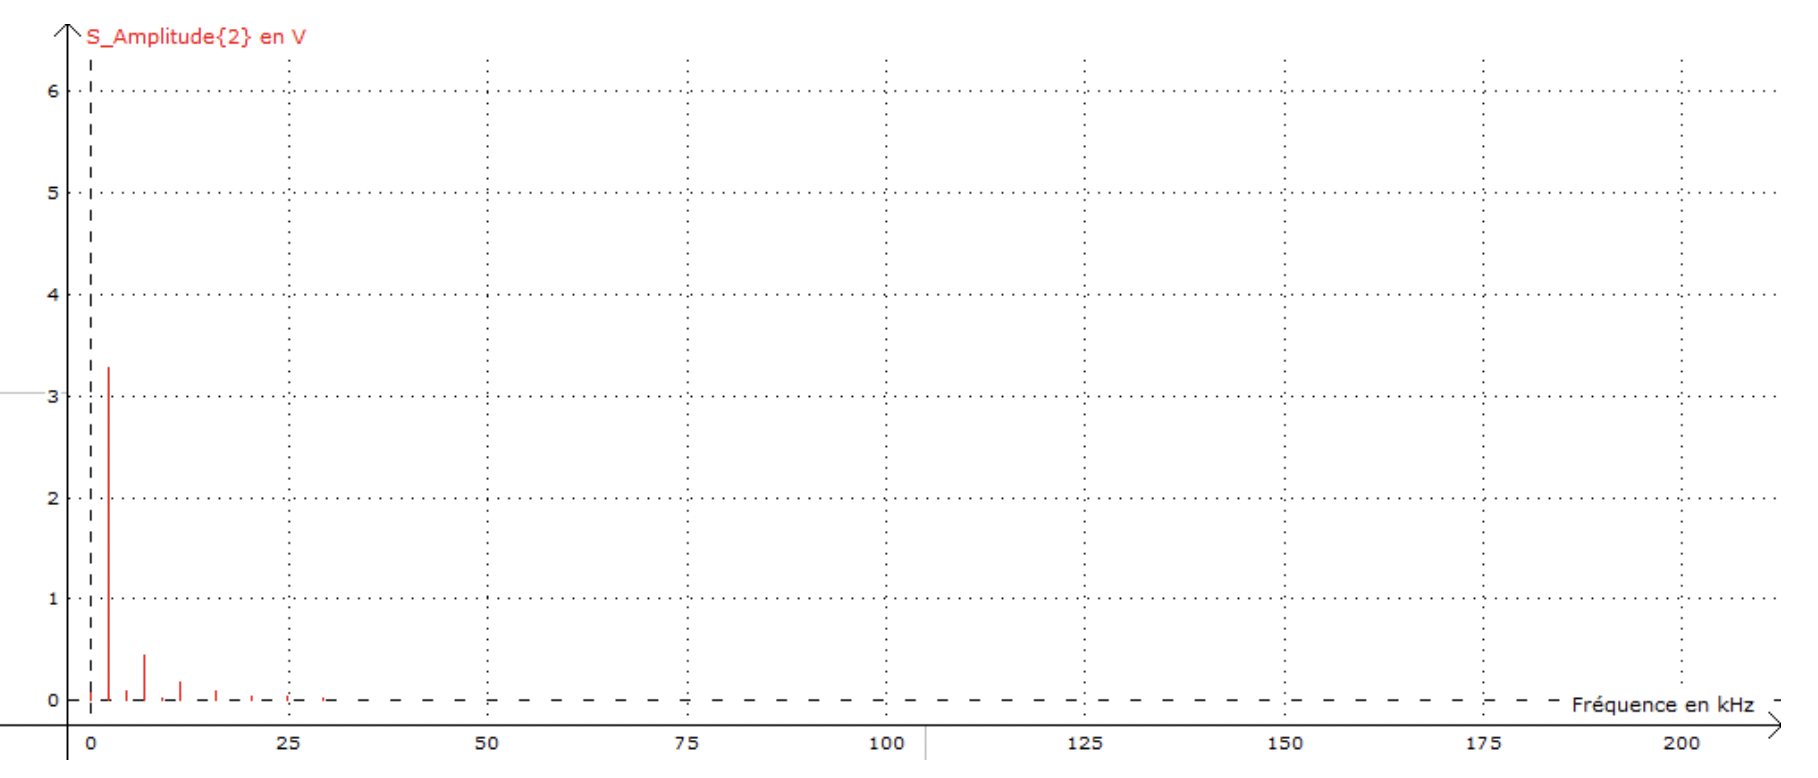
\includegraphics[scale=0.28]{filtre-actif-spectre-sortie-2250} 

\esp

Seuls le fondamental et les premiers harmoniques, ayant des fréquences dans la bande passante du filtre, vont être transmise : le filtre étant peu sélectif,  on obtient une sinusoïde à 2250 Hz (fondamental) déformée par les premiers harmoniques.

On peut aussi analyser le signal de sortie comme le début de la réponse à des échelons de tension en régime pseudo-périodique : le changement de créneau intervient alors que le régime permanent n'est pas atteint.
\esp

- Pour $f = 10\ \kilo\hertz$ on obtient les courbes temporelles :
\esp

\hspace{1cm}
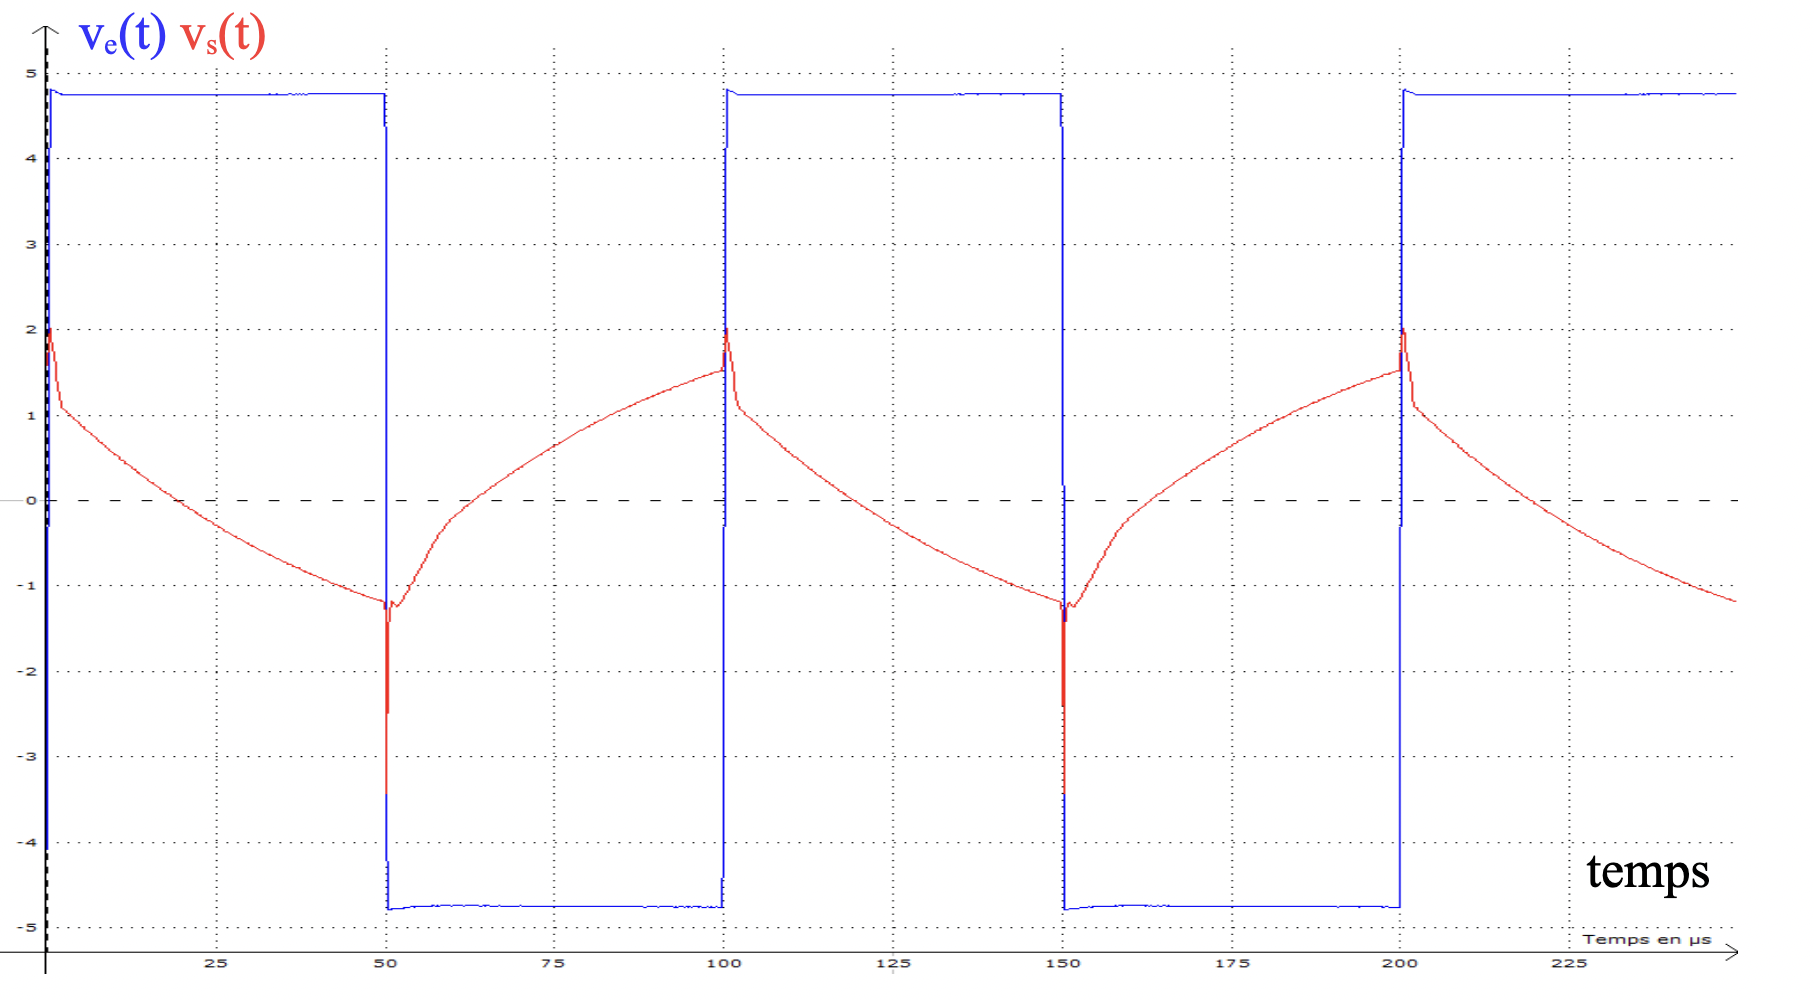
\includegraphics[scale=0.31]{filtre-actif-10000-t.png}
\esp

Spectres des signaux d'entrée et de sortie :


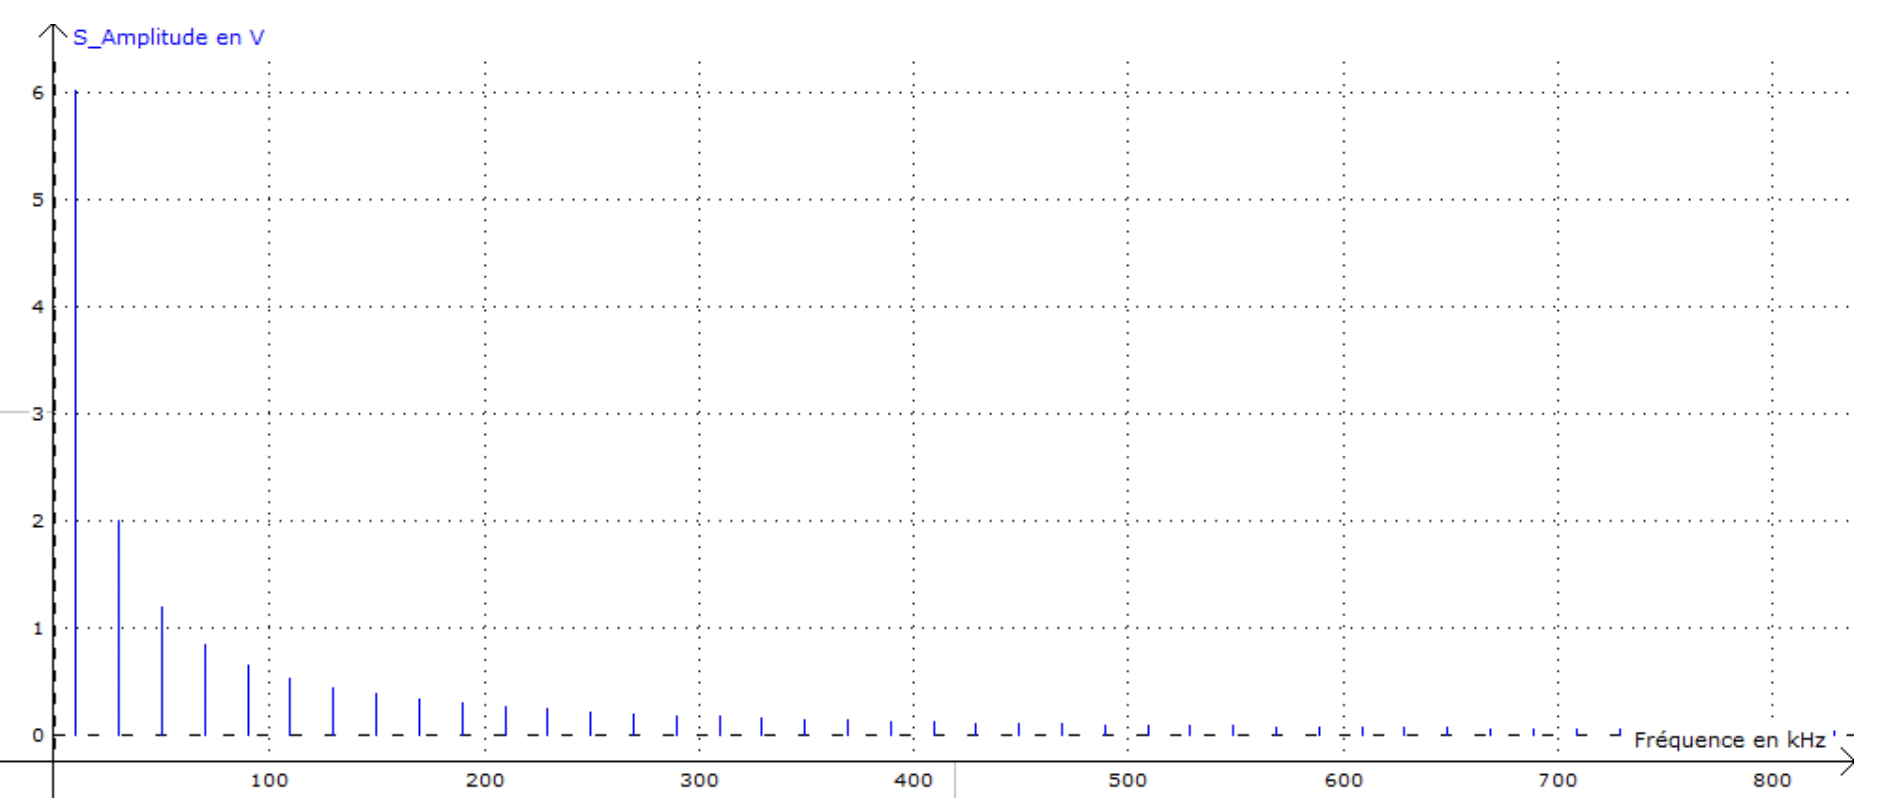
\includegraphics[scale=0.3]{filtre-actif-spectre-entree-10000} 

\hspace{-0.1cm}
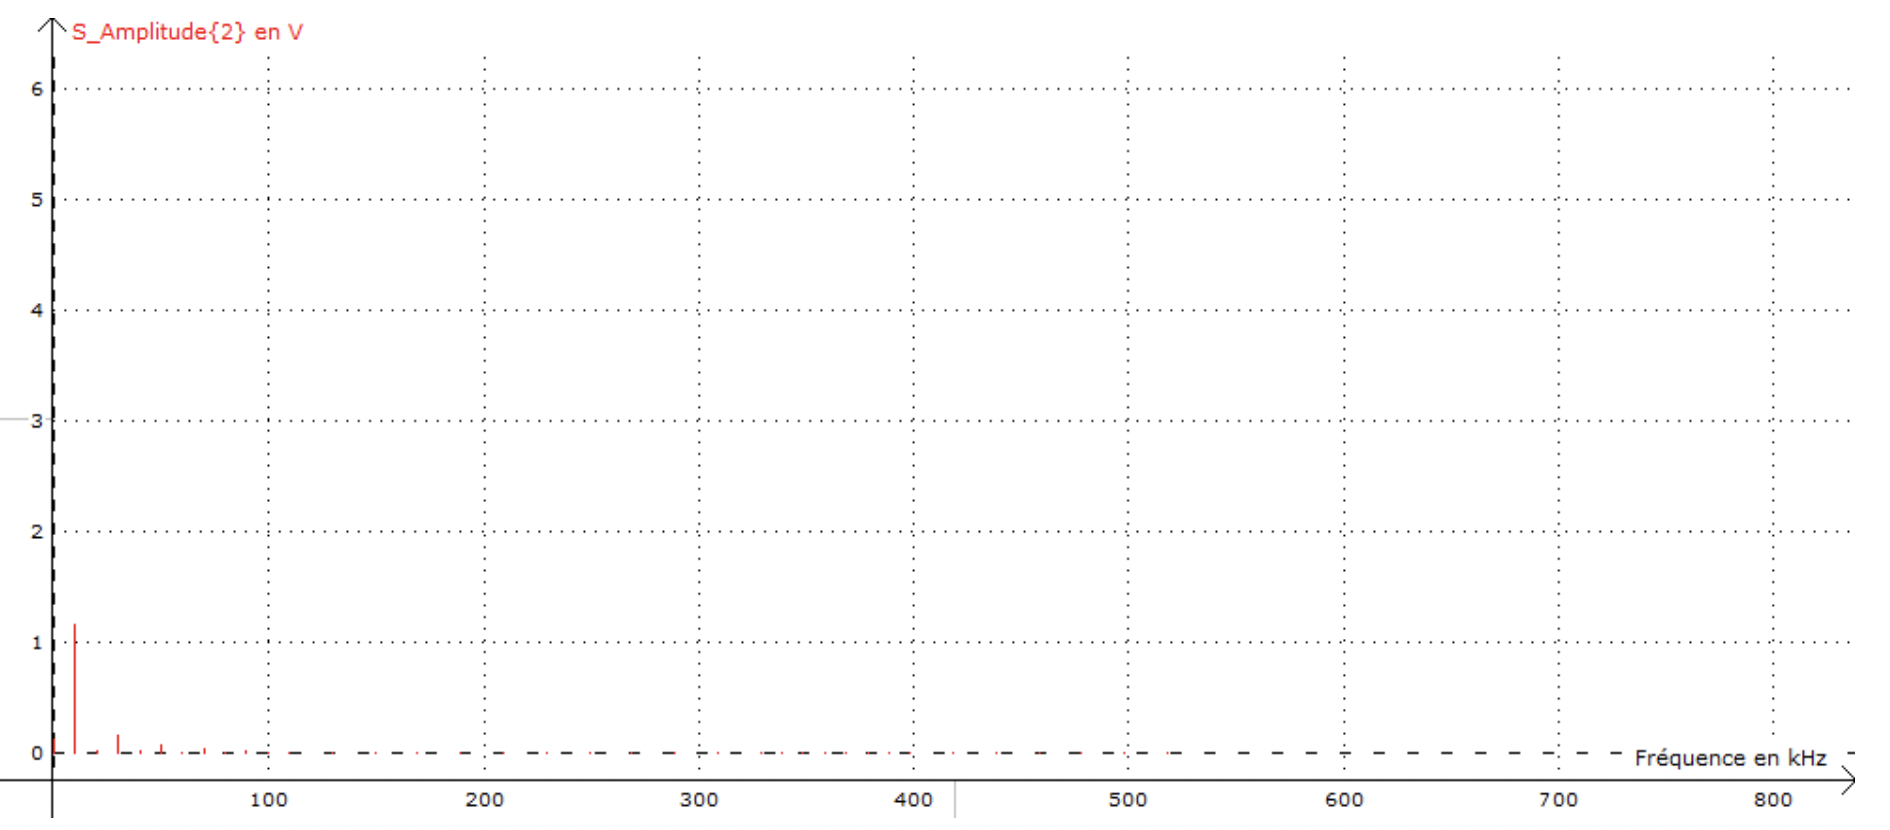
\includegraphics[scale=0.3]{filtre-actif-spectre-sortie-10000} 

\esp

Toutes les composantes du signal d'entrée  sont dans la pente à - 20 dB / décade du diagramme du gain du filtre : le signal d'entrée est intégré et le signal de sortie est proche d'un signal triangulaire.

On peut aussi analyser le signal de sortie comme le tout début de la réponse à des échelons de tension en régime pseudo-périodique : le changement de créneau intervient alors que le régime permanent n'est pas atteint.




\newpage

\begin{center}
\begin{LARGE}
\textbf{Annexe}
\end{LARGE}
\end{center}

\noi
• \textbf{Montage dérivateur.}
\esp

Circuit : 

\vspace{-0.5cm}
\hspace{2cm}
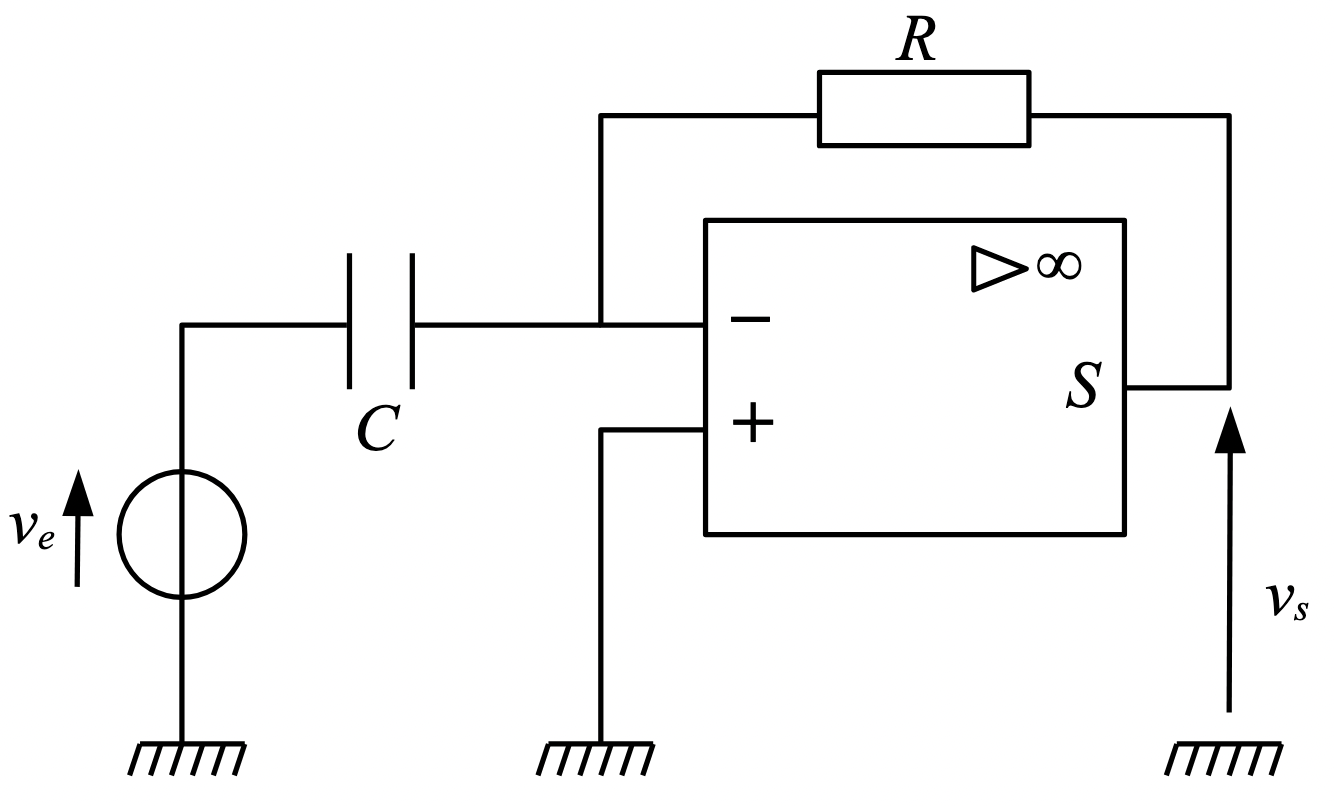
\includegraphics[scale=0.3]{E8-cours-0-derivateur.png}

\vspace{-0.2cm}
Calculs : 
\vspace{0.1cm}

- à l'entrée $E^+$ :  $\so{V}^+ = 0\ \volt$ ;
\vspace{0.1cm}

- loi des nœuds en terme de potentiel à l'entrée $E^-$ : $\d jC\omega (\so{v}_e - \so{V}^-) + \frac{\so{v}_s}{R} = 0$

soit $\d \so{V}^- = \frac{jC\omega \so{v}_e + \frac{\so{v}_s}{R}}{jC\omega + \frac{1}{R}}$ ;
\vspace{0.1cm}

- boucle de rétroaction sur l'entrée $E^-$ : l'amplificateur fonctionne en régime linéaire donc $\so{V}^+ = \so{V}^-$ donc $\d jC\omega\so{v}_e + \frac{\so{v}_s}{R} = 0$ ;
\vspace{0.1cm}

- on déduit $\d \so{v}_s = -jRC\omega \so{v}_e$ donc $\d v_s(t) = -RC\frac{dv_e(t)}{dt}$.
\esp

\noi
• \textbf{Calculs sur le filtre passe-bande abordé dans le cours.}
\vspace{0.1cm}

- à l'entrée $E^+$ :  $\so{V}^+ = 0\ \volt$ ;
\vspace{0.1cm}

- loi des nœuds en terme de potentiel au nœud $A$ :

\vspace{0.1cm} 
$\d \frac{\so{v}_e - \so{V}_A}{R} + \frac{0 - \so{V}_A}{R} + jC\omega (\so{V}^- - \so{V}_A) + jC\omega (\so{v}_s - \so{V}_A) = 0$
\vspace{0.1cm}

soit $\d \so{V}_A = \frac{\frac{\so{v}_e}{R} + jC\omega \so{v}_s}{\frac{2}{R} + 2jC\omega}$ car $\so{V}^- = \so{V}^+ = 0\ \volt$ ;
\vspace{0.1cm}

- loi des nœuds en terme de potentiel à l'entrée inverseuse $E^-$ : 

\vspace{0.1cm} 
$\d jC\omega (\so{V}_A - \so{V}^-) + \frac{\so{v}_s - \so{V}^-}{R}  = 0$ soit $\d \so{V}_A = -\frac{1}{jRC\omega}\so{v}_s$ car $\so{V}^- = 0\ \volt$.
\vspace{0.1cm}

- on associe les 2 relations trouvées : $\d -\frac{1}{jRC\omega}\so{v}_s =  \frac{\frac{\so{v}_e}{R} + jC\omega \so{v}_s}{\frac{2}{R} + 2jC\omega}$ soit
\vspace{0.1cm}

$ -\left(\frac{2}{R} + 2jC\omega \right) \so{v}_s = jRC\omega \left(\frac{\so{v}_e}{R} +jC\omega \so{v}_s\right)$ soit $\d - (2 + 2jRC\omega) -R^2C^2\omega^2)\so{v}_s
 = jRC\omega \so{v}_e$.
 \vspace{0.1cm}
 
 On déduit : $\d \so{H} = \frac{\so{v}_s}{\so{v}_e} = \frac{-jRC\omega}{2-R^2C^2\omega^2 + 2jRC\omega} = \frac{-1/2}{1 + \frac{1}{jRC\omega} + \frac{jRC\omega}{2}}$
\vspace{0.1cm}

donc $\d \so{H} = \frac{-1/2}{1 + \frac{j}{\sqrt{2}}\left( \frac{RC\omega}{\sqrt{2}} -\frac{\sqrt{2}}{RC\omega}\right)} = \frac{H_0}{1 + jQ\left(\frac{\omega}{\omega_0}- \frac{\omega_0}{\omega}\right)}$ en posant
\vspace{0.1cm}

$\d \omega_0 = \frac{\sqrt{2}}{RC} = 2\pi f_0$ soit $\d f_0 = \frac{1}{\sqrt{2}\pi RC}$, $H_0 = -1/2$ et $Q = \frac{1}{\sqrt{2}}$.

\newpage


\begin{center}
\begin{LARGE}
\textbf{Réponses aux tests}
\end{LARGE}
\end{center}


\hspace{-0.5cm}\rule{\linewidth}{.5pt}

\esp
\noi
\ovalbox{\textbf{Test 1}}
\esp

\noi 
• Le diagramme de Bode est celui d'un filtre passe-bas d'ordre 1 (pente à -20 dB/décade), avec $f_c$ de l'ordre de $0,5.10^5\ \hertz = 50\ \kilo\hertz$.

Oscillo 5 n'effectue des mesures cohérentes que jusqu'à 80 kHz donc il vaut mieux mesurer $f_c$ avec $G_{\deci\bel}(f_c) = G_{\deci\bel max} - 3\ \deci\bel$.
\esp

\noi
• L'ALI idéal présenterait un diagramme de Bode pour le gain horizontal. L'ALI réel présente un problème pour les hautes fréquences (chute du gain).

\hspace{-0.5cm}\rule{\linewidth}{.5pt}

\esp
\noi
\ovalbox{\textbf{Test 2}}
\esp

\noi 
• $\so{V}^+ = 0\ \volt$.
\esp

\noi
• La loi des nœuds en terme de potentiel à l'entrée inverseuse donne :
\vspace{0.1cm}

$\d \so{V}^- = \frac{\frac{\so{v}_e}{R} +jC\omega\so{v}_s}{\frac{1}{R} + jC\omega} = \frac{\so{v}_e + jRC\omega \so{v}_s}{1 + jRC\omega}$.
\esp

\noi
• Boucle de rétroaction sur l'entrée inverseuse : l'ALI fonctionne en régime linéaire donc $\so{V}^+ = \so{V}^-$ donc $\so{V}^- = 0\ \volt$ d'où $\so{v_e} + jRC\omega \so{v}_s = 0$.
\esp

\noi
• On déduit : $\d \so{v}_s = -\frac{1}{jRC\omega}\so{v}_e$ d'où $\d v_s(t) = -\frac{1}{RC}\int v_e(t) dt$.

\hspace{-0.5cm}\rule{\linewidth}{.5pt}

\esp
\noi
\ovalbox{\textbf{Test 3}}
\esp

\noi 
$\omega \rightarrow 0$ : on va avoir $G \rightarrow \infty$ d'où saturation en sortie de l'ALI.

\hspace{-0.5cm}\rule{\linewidth}{.5pt}

\esp
\noi
\ovalbox{\textbf{Test 4}}
\esp

\noi 
$\d V^+ = 0\ \volt$ ; $\d V^- = \frac{\dfrac{v_e}{R} + \dfrac{v_s}{R'}}{\dfrac{1}{R} + \dfrac{1}{R'}}$ ; $V^+ = V^-$ donne $\d v_s = -\frac{R'}{R}v_e$.

\hspace{-0.5cm}\rule{\linewidth}{.5pt}

\esp
\noi
\ovalbox{\textbf{Test 5}}
\esp

\noi 
$v_e = Ri_e$ donc $\so{Z}_e = R$.
 

\end{document}
